%% SPDX-License-Identifier: CC-BY-4.0
%% SPDX-FileCopyrightText: 2026 Serge TABE DJATO
% !TeX program = xelatex
%% ============================================================
%% IntrepidCore — Livre blanc ICES v3.0
%% Le sceau de responsabilité de l'ingénierie publique.
%% v2 -> v3 : chaîne de garde (Manifeste de Projet), hiérarchie des
%% preuves de terrain, horodatage en deux paliers, cérémonie de clé
%% racine à seuil, agilité cryptographique/post-quantique, réponse à
%% incident, nuance sur la faute dolosive, refus du hash de build
%% comme parade au passager clandestin, spécification en annexe
%% (JSON Schema, table de précision, format de révocation).
%% ============================================================
\documentclass[11pt,a4paper]{article}
\usepackage[a4paper,top=2.4cm,bottom=2.6cm,left=2.5cm,right=2.5cm]{geometry}
\usepackage[french]{babel}\usepackage{csquotes}\usepackage{fontspec}\usepackage{microtype}
\IfFontExistsTF{Times New Roman}{\setmainfont{Times New Roman}}{\setmainfont{TeX Gyre Termes}}
\usepackage{amsmath}\usepackage{amssymb}\usepackage{graphicx}\usepackage{booktabs}\usepackage{array}
\usepackage{colortbl}\usepackage{tabularx}\usepackage{float}\usepackage{enumitem}
\usepackage{titlesec}\usepackage{xcolor}\usepackage{fancyhdr}\usepackage{tcolorbox}
\usepackage{tikz}\usetikzlibrary{shapes.geometric,arrows.meta,positioning,calc,decorations.pathreplacing}
\tcbuselibrary{skins}\usepackage{hyperref}\usepackage{listings}
\usepackage[style=ieee,backend=biber]{biblatex}\addbibresource{ICES-whitepaper-v3-bibliographie.bib}

% Police Excalidraw (Virgil) pour le texte des figures TikZ — élément de charte IntrepidCore
\newfontfamily\excalifont[Path=../../font/,AutoFakeBold=2.5]{Virgil.ttf}
\lstdefinestyle{icesjson}{basicstyle=\ttfamily\scriptsize\color{grisfonce},
  breaklines=true, columns=fullflexible, keepspaces=true, frame=single,
  rulecolor=\color{intrepid!40}, backgroundcolor=\color{intrepid!3},
  showstringspaces=false, xleftmargin=3pt, xrightmargin=3pt}

\definecolor{intrepid}{RGB}{0,57,107}\definecolor{accent}{RGB}{213,93,36}
\definecolor{cyanIC}{RGB}{0,196,212}\definecolor{vertAtlas}{RGB}{64,145,108}
\definecolor{rowgray}{RGB}{240,240,240}\definecolor{rouge}{RGB}{178,34,34}
\definecolor{grisfonce}{RGB}{40,40,40}

\hypersetup{hidelinks, pdfauthor={Serge TABE DJATO},
  pdftitle={ICES v3.0 — Le sceau de responsabilité de l'ingénierie publique},
  pdfsubject={Standard ouvert de preuve cryptographique et d'attribution pour l'ingénierie hydraulique}}

\newcommand{\mylogo}{
\includegraphics[height=2cm]{../assets/logo}}
\newcommand{\headerblock}{%
  \noindent\begin{minipage}[c]{0.45\linewidth}\mylogo\end{minipage}\hfill
  \begin{minipage}[c]{0.52\linewidth}\raggedleft
    {\footnotesize\color{gray}IntrepidCore \textperiodcentered\ Livre blanc technique \textperiodcentered\ v3.0 \textperiodcentered\ Juillet~2026}%
  \end{minipage}\par\vspace{5pt}\rule{\linewidth}{1pt}\vspace{0.4cm}}

\newtcolorbox{icesbox}[2][]{enhanced, colback=#2!8!white, colframe=#2, boxrule=0.6pt,
  left=6pt, right=6pt, top=5pt, bottom=5pt, fonttitle=\bfseries\small\color{#2}, title={#1}}
\newtcolorbox{termbox}[1][]{enhanced, colback=grisfonce!95!white, colframe=grisfonce, boxrule=0.6pt,
  left=6pt, right=6pt, top=5pt, bottom=5pt, fontupper=\ttfamily\small\color{white}, title={#1},
  fonttitle=\bfseries\small\color{white}, coltitle=white}

\setlength{\parindent}{0pt}\setlength{\parskip}{6pt plus 1pt minus 0.5pt}
\titleformat{\section}{\normalfont\fontsize{13}{15}\bfseries\color{intrepid}}{\thesection.}{0.6em}{}
\titleformat{\subsection}{\normalfont\fontsize{11}{13}\bfseries\color{accent}}{\thesubsection}{0.5em}{}
\titlespacing{\section}{0pt}{14pt}{6pt}

\pagestyle{fancy}\fancyhf{}
\fancyhead[L]{\small\color{intrepid}\textsc{IntrepidCore} \textemdash\ ICES v3.0}
\fancyhead[R]{\small\thepage}
\fancyfoot[C]{\small\textit{Livre blanc technique \textemdash\ \textcopyright{} IntrepidCore 2026}}
\renewcommand{\headrulewidth}{0.4pt}\renewcommand{\footrulewidth}{0.4pt}

\newcommand{\padlock}[2][1]{%
  \begin{tikzpicture}[scale=#1]
    \draw[line width=1.4pt, color=#2] (-0.35,0) rectangle (0.35,-0.55);
    \draw[line width=1.4pt, color=#2] (-0.22,0) arc (180:0:0.22) ;
    \fill[color=#2] (-0.06,-0.22) rectangle (0.06,-0.4);
  \end{tikzpicture}}

%% ══════════════════════════════════════════════════════════════
\begin{document}

%% ─────────────────────────────────────────────────────────────
%% COUVERTURE
\thispagestyle{empty}
\headerblock

\begin{center}
  {\fontsize{16}{19}\bfseries\color{intrepid} ICES}\\[6pt]
  {\fontsize{13}{16}\bfseries Le sceau de responsabilité de l'ingénierie publique}\\[6pt]
  {\fontsize{10.5}{13}\normalfont\color{gray} Lier cryptographiquement chaque décision d'infrastructure à son auteur.\\Spécification et doctrine d'un standard ouvert pour l'espace UEMOA.}\\[3pt]
  {\footnotesize\color{gray} IntrepidCore \textperiodcentered\ Version 3.0 \textperiodcentered\ Juillet 2026}
\end{center}
\vspace{0.3cm}

\begin{icesbox}[Résumé]{intrepid}
Une note de calcul d'ingénierie hydraulique fixe le diamètre d'une conduite, la pression qu'elle doit supporter, la capacité d'un château d'eau. Entre l'étude et la mise en service, ce document traverse trois transitions où son contenu peut être remplacé sans que la modification laisse de trace exploitable. Ce livre blanc présente ICES (IntrepidCore Engineering Standard), un standard ouvert de scellement cryptographique pour ces documents. La position défendue ici est délibérément bornée~: ICES ne rend pas la fraude physique impossible, et ce document explique pourquoi une telle promesse serait fausse. ICES rend une décision d'ingénierie \textbf{attribuable, datée et non répudiable}, et connecte cette attribution aux mécanismes de responsabilité contractuelle et assurantielle qui existent déjà dans le droit de la commande publique UEMOA et le Code CIMA. Le document expose la spécification technique, les limites explicites du mécanisme, la doctrine de gouvernance retenue et le modèle économique qui en découle.
\end{icesbox}

\newpage
\tableofcontents
\thispagestyle{empty}
\newpage

%% ═════════════════════════════════════════════════════════════
\section{Introduction et contexte}\label{sec:intro}

\subsection{Le problème de fond~: une décision d'ingénierie n'est pas attribuable}

La conception d'un réseau d'eau potable repose sur une note de calcul hydraulique qui fixe les diamètres de canalisation, les pressions de service, les volumes de stockage. Un maître d'ouvrage public, un bailleur de fonds, une compagnie d'assurance décennale s'appuient sur ce document pour engager des fonds, valider un chantier, ou couvrir un risque sur dix ans. Aujourd'hui, ce document ne porte aucune garantie d'origine~: rien ne permet de savoir, avec certitude, qui l'a produit, à quel instant, ni si le fichier remis à la réception est identique à celui validé à l'étude.

Le cycle de vie d'un marché de travaux comporte trois transitions où cette garantie disparaît.

\begin{enumerate}[leftmargin=1.4em, itemsep=2pt]
  \item \textbf{Étude~$\to$~Exécution.} L'entreprise adjudicataire produit ses propres études d'exécution. Une altération du coefficient de rugosité ou des hypothèses de débit permet de justifier un diamètre de canalisation inférieur, moins coûteux. Faute de moyen de vérification rapide, le Maître d'Œuvre appose son visa \enquote{Bon Pour Exécution} sur un dossier qui s'écarte silencieusement de l'enveloppe d'origine.
  \item \textbf{Exécution~$\to$~Chantier.} Même quand l'étude d'exécution reste fidèle à l'APD, la pose peut ne pas l'être~: substitution de classe de pression, contrefaçon de raccords et de vannes, modification non déclarée de la profondeur d'enfouissement. Les bordereaux de livraison sont falsifiés, les tranchées remblayées, la preuve matérielle disparaît.
  \item \textbf{Chantier~$\to$~Réception.} Le \enquote{Dossier de Récolement}, censé documenter fidèlement l'ouvrage réel, est fréquemment une recopie des plans initiaux, sans intégrer les déviations survenues en chantier. Une fois la réception prononcée, la déconnexion entre l'infrastructure documentée et l'infrastructure enterrée devient pratiquement irréversible.
\end{enumerate}

Nous appelons cette discontinuité l'\textbf{Air Gap APD-EXE}. Elle n'est pas une hypothèse~: elle correspond à un motif documenté dans les rapports d'audit de plusieurs autorités de régulation des marchés publics de la sous-région, qui constatent de façon répétée l'absence de procès-verbaux de réception des matériaux et l'insuffisance du suivi de l'exécution~\cite{arcop_togo_2015,arcop_senegal_2022}.

\begin{icesbox}[Scénario illustratif, à valeur pédagogique]{rouge}
Un réseau d'adduction dessert un quartier de Lomé. L'APD prescrit une conduite PEHD PN16 de 110\,mm sur le tronçon principal. L'entreprise adjudicataire pose du PN10, moins coûteux d'environ 30\,\%. Le Dossier de Récolement recopie les plans d'origine sans mention de cette substitution. La réception est prononcée. À la quatrième année d'exploitation, la conduite éclate sous une surpression que le PN10 ne pouvait pas supporter. Sans document attribuable, l'expertise post-sinistre doit reconstituer, par expertise contradictoire, qui de l'étude, de l'exécution ou de la pose porte la responsabilité. Ce document propose un mécanisme qui rend cette reconstitution immédiate plutôt que contentieuse, sans prétendre que la substitution elle-même serait devenue impossible. La section~\ref{sec:oracle} explique précisément où s'arrête cette garantie.
\end{icesbox}

\begin{figure}[H]\centering
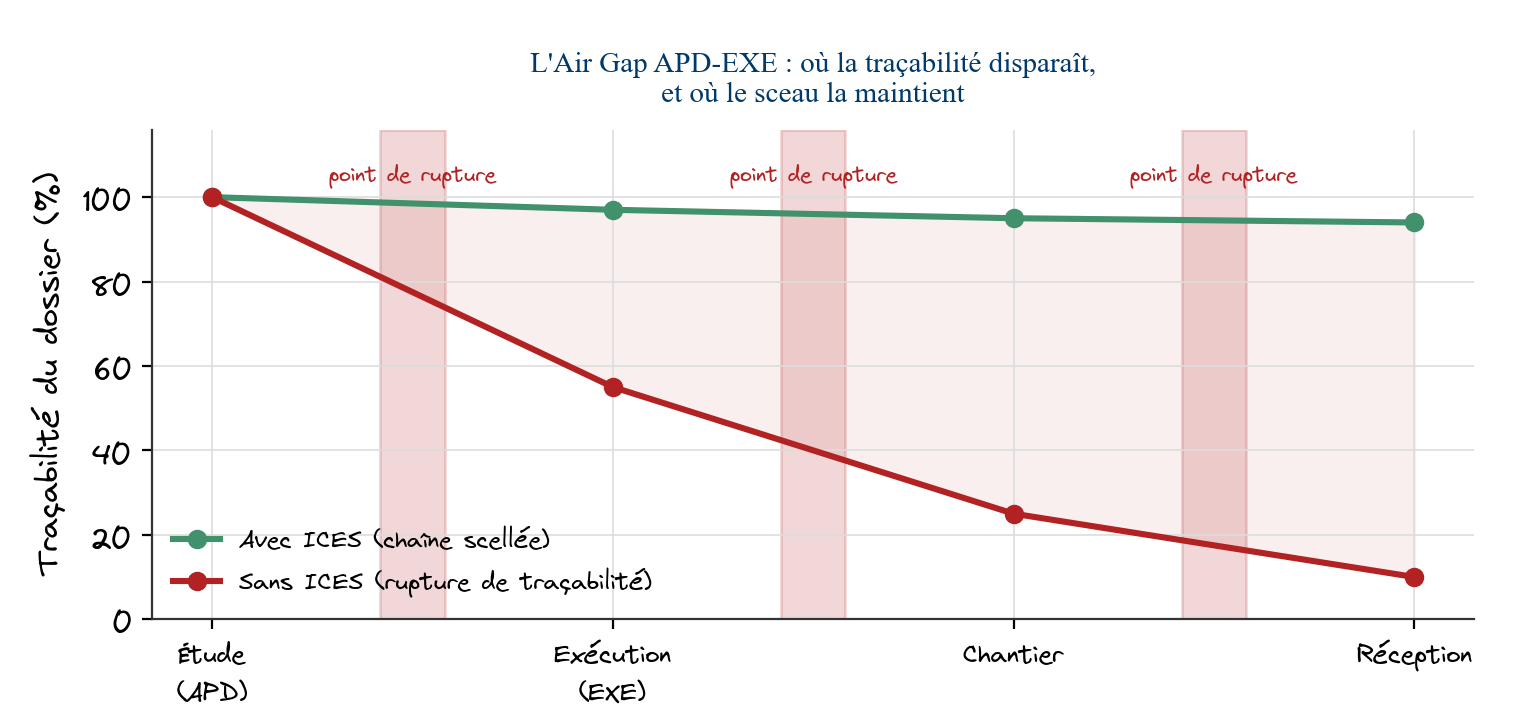
\includegraphics[width=0.86\linewidth]{figures/fig_airgap.png}
\caption{La traçabilité d'un dossier au fil des phases d'un marché de travaux. Sans mécanisme de scellement, elle s'effondre à chaque transition (études d'exécution, chantier, récolement)~; un dossier scellé et attribuable la maintient à chaque étape.}
\end{figure}

\subsection{Contexte de marché}

Une partie substantielle des notes de calcul circulant dans la commande publique ouest-africaine est produite sous tableur généraliste, sans traçabilité des hypothèses ni des formules, un format qu'aucun tiers ne peut auditer a posteriori sans refaire entièrement le calcul. Ce déficit d'auditabilité, et non le taux d'usage de logiciels sans licence dans la région, est le problème qu'adresse ICES~: un calcul produit sous un logiciel sans licence peut être scellé avec la même intégrité qu'un calcul produit sous licence, et un calcul produit sous licence peut tout aussi bien dissimuler une fraude en aval. Le lien, indirect, entre ce marché du logiciel et l'adoption d'ICES est traité en section~\ref{sec:economie}~; il n'est pas la thèse de ce document.

\subsection{Portée et non-portée de ce document}

Ce document spécifie un mécanisme de preuve cryptographique, sa doctrine de gouvernance, et une spécification technique de mise en œuvre (annexe~\ref{sec:annexe}). Il ne prétend pas que ce mécanisme élimine la fraude d'ingénierie, ni qu'il dispense d'inspection physique, ni qu'il remplace le contrôle technique réglementaire~; la section~\ref{sec:limites} énonce explicitement ce qu'ICES ne fait pas. Le lecteur non technicien peut suivre le fil narratif (contexte, gouvernance, responsabilité juridique, limites)~; le lecteur cryptographe ou auditeur de sécurité trouvera l'exposé formel dans les sections techniques (anatomie du sceau, maillon de confiance, chaîne de garde, sécurité opérationnelle, déterminisme) et la spécification en annexe.

%% ═════════════════════════════════════════════════════════════
\section{Pourquoi les réponses existantes ne suffisent pas}\label{sec:reponses}

Trois familles de réponses existent aujourd'hui. Aucune ne referme, seule, l'Air Gap.

\textbf{L'audit a posteriori} (missions de contrôle technique, audits des autorités de régulation, procédures de saisie-contrefaçon) intervient après le remblaiement de la tranchée, quand la preuve matérielle a disparu. Engager une procédure contre une multitude de petites structures dispersées sur un territoire représente, en pratique judiciaire, un coût souvent supérieur à ce que la fraude fait perdre à l'administration.

\textbf{La signature symétrique auto-certifiante} donne l'illusion d'une preuve sans en être une. Un design de scellement où la clé publique de vérification est embarquée dans le document lui-même ne prouve que la possession d'une clé au moment de la signature, jamais l'identité ou la légitimité du signataire~: n'importe qui peut générer sa propre paire de clés, resigner un document modifié, et obtenir une vérification techniquement positive. C'est un défaut de conception documenté dans la littérature de gestion de clés~\cite{nist80057} sous le nom de \emph{trust-on-first-use} sans ancrage externe, et il constitue précisément la raison pour laquelle ICES sépare la vérification de signature (section~\ref{sec:anatomie}) de la vérification de confiance (section~\ref{sec:confiance}).

\textbf{La boîte noire propriétaire} déplace le problème sans le résoudre~: elle demande de faire confiance à l'éditeur du logiciel plutôt qu'à l'auteur du calcul. Aucun tiers ne peut auditer indépendamment ce qui se passe à l'intérieur, et l'architecture reste dépendante d'un fournisseur unique, un choix difficile à justifier pour un État qui engage des fonds publics ou empruntés sur plusieurs décennies. Un changement de conditions commerciales ou une simple interruption de service suffit à rendre le dispositif de preuve inaccessible au moment où un contentieux en aurait le plus besoin.

\begin{table}[H]\centering\small
\caption{Trois approches, trois garanties différentes}
\begin{tabularx}{\linewidth}{@{}p{3.6cm}XXX@{}}
\toprule
& \textbf{Audit a posteriori} & \textbf{Boîte noire propriétaire} & \textbf{ICES} \\
\midrule
Détection de l'altération & Après coup, si un contrôle a lieu & Non auditable par un tiers & Immédiate, par quiconque possède le fichier \\
Coût de vérification & Élevé (expertise, contentieux) & Nul pour l'éditeur, opaque pour le client & Nul, calcul local en quelques secondes \\
Fonctionne hors-ligne & Non & Non & Oui, par construction \\
Gouvernance & Neutre & Propriétaire, fournisseur unique & Cédée par phases (section~\ref{sec:gouvernance}) \\
\bottomrule
\end{tabularx}
\end{table}

\begin{center}
\begin{tikzpicture}[scale=1]
  \draw[-{Latex[length=2.5mm]}, thick, gray] (0,0) -- (8.2,0) node[right, font=\excalifont\small] {Coût de vérification};
  \draw[-{Latex[length=2.5mm]}, thick, gray] (0,0) -- (0,5.2) node[above, font=\excalifont\small] {Détection de l'altération};
  \node[font=\excalifont\footnotesize\color{gray}] at (0.9,-0.4) {faible};
  \node[font=\excalifont\footnotesize\color{gray}] at (7.3,-0.4) {élevé};
  \node[font=\excalifont\footnotesize\color{gray}, rotate=90] at (-0.4,0.9) {tardive};
  \node[font=\excalifont\footnotesize\color{gray}, rotate=90] at (-0.4,4.3) {immédiate};
  \node[draw=intrepid, thick, rounded corners, fill=intrepid!8, align=center, font=\excalifont\small] at (2.6,4.4) {Audit\\a posteriori};
  \node[draw=accent, thick, rounded corners, fill=accent!8, align=center, font=\excalifont\small] at (1.4,0.9) {Boîte noire\\propriétaire};
  \node[draw=vertAtlas, thick, rounded corners, fill=vertAtlas!8, align=center, font=\excalifont\small] at (1.4,4.4) {ICES};
\end{tikzpicture}
\end{center}
\begin{center}\footnotesize\color{gray}Positionnement qualitatif des trois approches sur deux axes~: coût de vérification et délai de détection.\end{center}

%% ═════════════════════════════════════════════════════════════
\section{Les trois garanties d'ICES, et où elles s'arrêtent}\label{sec:garanties}

La faiblesse la plus commune d'un discours sur la preuve cryptographique consiste à laisser une garantie forte prêter sa crédibilité à des garanties qu'elle ne peut pas fournir. ICES distingue explicitement trois niveaux de garantie, de nature différente, et refuse d'en laisser un se substituer aux deux autres.

\begin{table}[H]\centering\small
\caption{Les trois garanties et leur nature}
\begin{tabularx}{\linewidth}{@{}p{3.4cm}Xp{2.4cm}@{}}
\toprule
\textbf{Garantie} & \textbf{Ce qu'elle établit} & \textbf{Force} \\
\midrule
Intégrité du calcul & Le résultat scellé provient de ces entrées, via ce moteur, sans altération depuis la signature. & Absolue. Fondée sur des primitives cryptographiques standardisées et publiquement éprouvées (section~\ref{sec:anatomie}). \\
Attribution & Un acteur identifié, à une clé enrôlée par une autorité reconnue, a produit cette signature à un instant donné. & Conditionnelle à la gouvernance du registre de confiance (section~\ref{sec:confiance}). \\
Véracité physique & Le contenu scellé correspond à l'état réel de l'ouvrage sur le terrain. & \textbf{Nulle par construction.} Aucun mécanisme cryptographique ne peut établir ce lien (section~\ref{sec:oracle}). \\
\bottomrule
\end{tabularx}
\end{table}

\begin{figure}[H]\centering
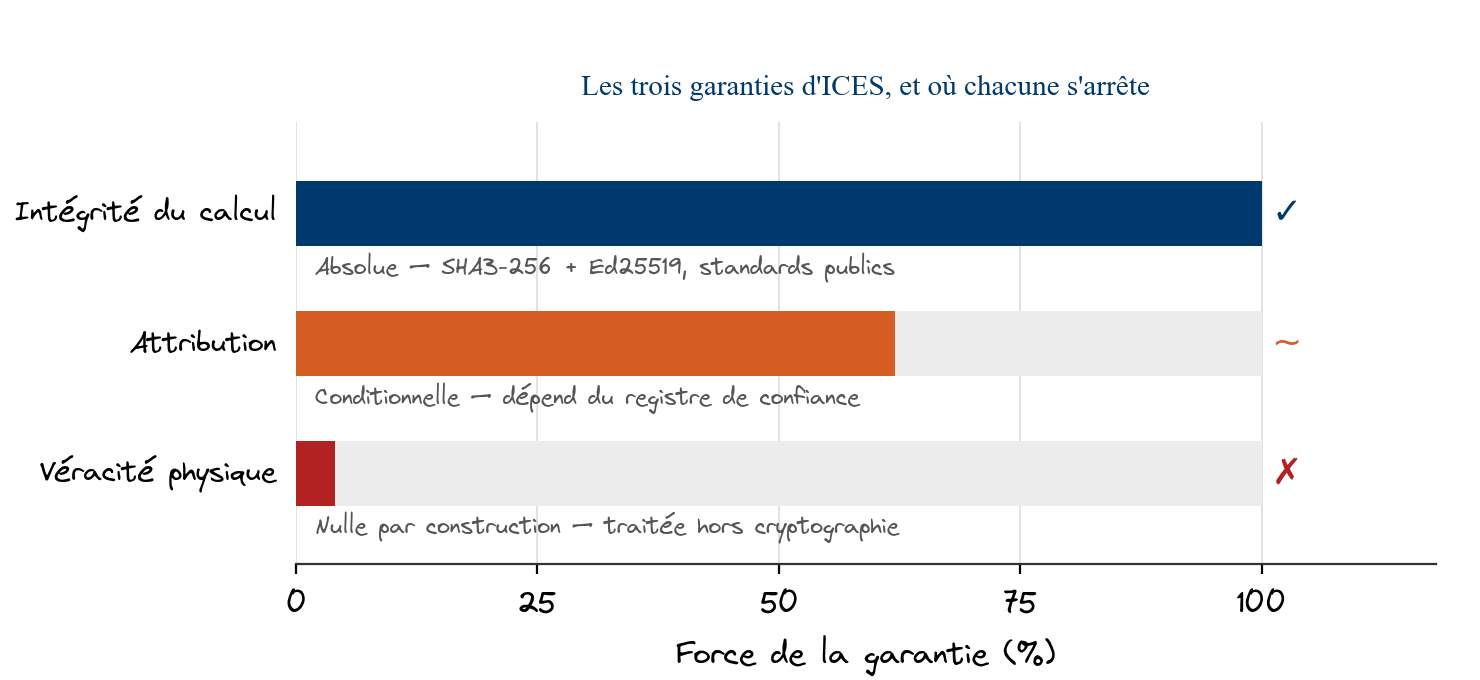
\includegraphics[width=0.82\linewidth]{figures/fig_guarantees.png}
\caption{La force respective des trois garanties. L'intégrité est absolue car elle ne dépend que de primitives publiques~; l'attribution est conditionnelle à la gouvernance du registre~; la véracité physique est nulle au niveau cryptographique et déléguée à d'autres mécanismes.}
\end{figure}

La troisième ligne de ce tableau distingue ICES de tout discours qui présenterait un sceau numérique comme une preuve de conformité physique. Elle est développée en détail en section~\ref{sec:oracle}, qui explique comment ICES traite ce qu'il ne peut pas prouver directement en le reliant à un tiers de confiance et à une chaîne de responsabilité, plutôt qu'en prétendant le résoudre par des mathématiques.

La conséquence pratique de ce cadrage se lit en une phrase~: ICES ne réduit pas à néant la possibilité d'une fraude, il en déplace le coût. Une fraude qui était, avant lui, dissimulable et déniable devient une altération détectable et une décision signée, attribuable à une personne nommée et opposable devant un juge ou un assureur.

\begin{figure}[H]\centering
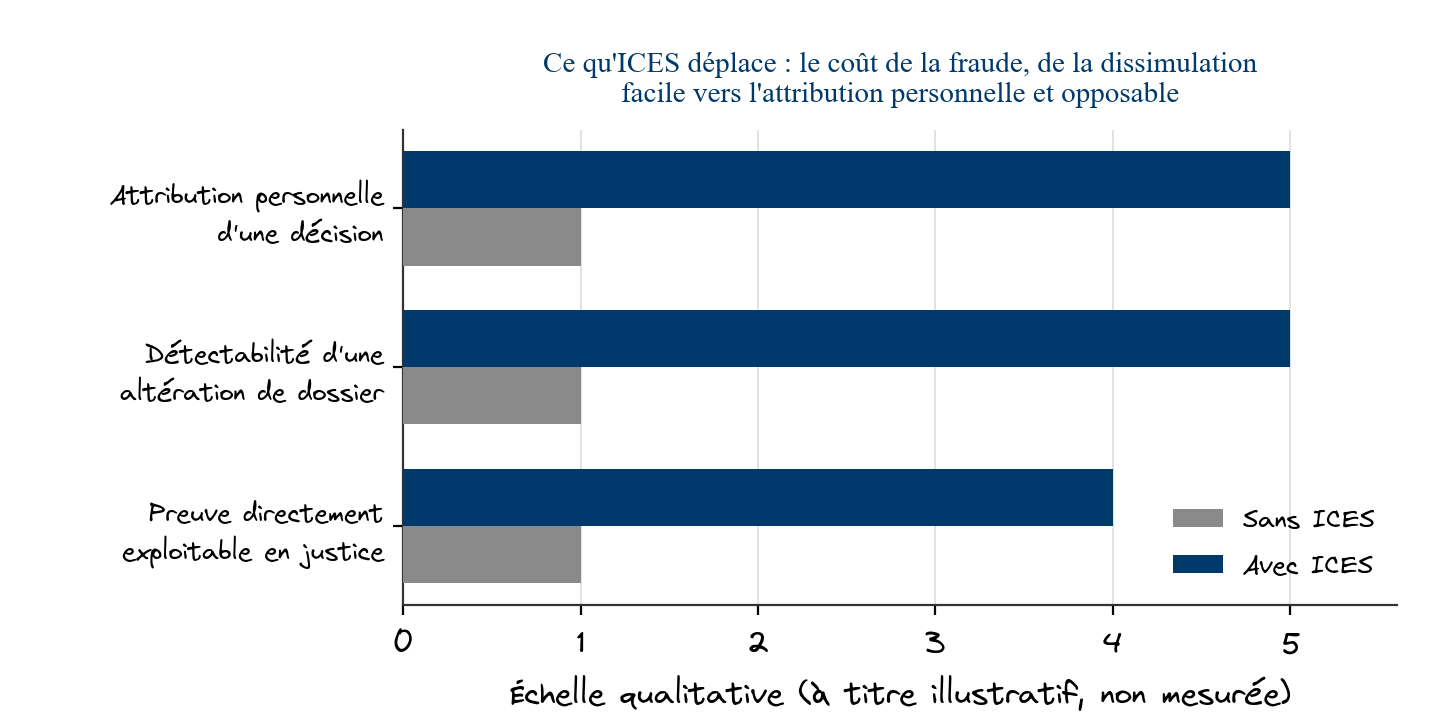
\includegraphics[width=0.80\linewidth]{figures/fig_fraudcost.png}
\caption{Ce qu'ICES modifie n'est pas la faisabilité de la fraude mais son coût~: l'attribution personnelle et la détectabilité d'une altération passent d'un niveau faible à un niveau élevé, ce qui alimente la chaîne de responsabilité juridique de la section~\ref{sec:juridique}.}
\end{figure}

%% ═════════════════════════════════════════════════════════════
\section{Gouvernance~: le précédent d'un standard ouvert, et son coût réel}\label{sec:gouvernance}

\subsection{Le précédent BIM/IFC et OCDS}

Lorsque le BIM s'est imposé dans la commande publique européenne, sous l'impulsion de la Directive 2014/24/UE~\cite{eu2014}, la crainte d'exclure les petits cabinets sans moyen d'acquérir des licences a été résolue en rendant obligatoire non pas un logiciel, mais un \textbf{format ouvert}, l'IFC, gouverné depuis par une organisation indépendante à but non lucratif que ni Autodesk ni aucun autre éditeur ne contrôle~\cite{buildingsmart}. Autodesk Revit et ArchiCAD sont deux outils \emph{compatibles IFC}, en concurrence l'un avec l'autre, sans que le format appartienne à aucun des deux. L'Open Contracting Data Standard suit le même principe pour la transparence des marchés publics, adopté par plus de cinquante gouvernements dont le Nigeria~\cite{ocds_nigeria} et la Tanzanie~\cite{ocds}~: une architecture de données publique, jamais un logiciel à acheter.

\subsection{La clause qui aurait recréé un monopole, et pourquoi elle est retirée}

Une première formulation possible d'une exigence contractuelle ICES consisterait à demander \enquote{l'intégrité de la modélisation et la validité de la licence du solveur utilisé}. Cette seconde exigence, la licence du solveur, recrée exactement le monopole que la première partie de la phrase cherche à éviter~: elle revient à imposer LCPI par la contrainte administrative, ce que l'article 48 de la Directive UEMOA sur les marchés publics interdit explicitement en prohibant toute exigence de marque ou de produit déterminé qui aurait pour effet de favoriser ou d'éliminer certaines entreprises~\cite{uemoa2005}. Une clause de ce type serait attaquable en recours contentieux devant l'Autorité de Régulation des Marchés Publics compétente et entraînerait potentiellement la nullité de la procédure de passation. La formulation retenue par ICES porte uniquement sur l'intégrité vérifiable du calcul, jamais sur l'identité de l'outil qui l'a produit.

\begin{icesbox}[Clause DAO recommandée]{vertAtlas}
\enquote{Les notes de calcul hydraulique remises au titre du présent marché devront être scellées par un mécanisme de preuve cryptographique vérifiable hors-ligne, conforme au standard ouvert ICES ou à tout protocole équivalent offrant un niveau de garantie mathématiquement comparable. La charge de la preuve de l'équivalence incombe au soumissionnaire.}
\end{icesbox}

Pour que cette clause de charge de la preuve ne devienne pas elle-même une barrière à l'entrée pour un petit bureau d'études, la gouvernance décrite ci-dessous prévoit un outil de référence gratuit qui rend la conformité atteignable sans achat d'aucune licence commerciale.

\subsection{Ce que la cession de gouvernance coûte réellement}

Publier une spécification ouverte n'a de valeur juridique et commerciale que si l'entité qui édite le standard ne le contrôle pas seule. Or cette cession a un coût réel, qu'il convient de chiffrer plutôt que d'euphémiser.

\textbf{Ce qui est perdu.} Le droit de modifier unilatéralement la spécification pour avantager LCPI~; une voix formelle égale accordée aux concurrents dans l'organe de gouvernance~; la vitesse du contrôle unilatéral, remplacée par la lenteur du consensus à mesure que l'organe grandit.

\textbf{Ce qui est conservé.} Le solveur stochastique LCPI, produit commercial distinct du standard, reste propriétaire~; la position d'auteur de l'implémentation de référence, qui dans les faits oriente durablement l'évolution technique du standard, indépendamment des règles formelles de vote~; la marque de conformité \enquote{ICES-Certified} et la suite de tests qui la définit (section~\ref{sec:conformite}), qui peuvent rester sous contrôle d'IntrepidCore même après cession de la spécification elle-même, sur le modèle de la certification USB-IF ou Wi-Fi Alliance~; la position de premier entrant sur l'intégration du registre de confiance et sur la couche de services associée.

Le premier droit perdu, celui de contrôler unilatéralement la spécification, est celui dont la perte est la condition de la valeur du standard~: un format qu'IntrepidCore contrôle seule seul reste, en droit, un format propriétaire, et la défense \enquote{ou équivalent} de l'article 48 ne tient que si ce contrôle n'existe pas. Le coût net de la cession se réduit donc, pour l'essentiel, à un ralentissement du rythme d'évolution du standard une fois la gouvernance élargie, contre l'acquisition d'une légitimité juridique que le contrôle unilatéral ne peut structurellement pas produire.

\subsection{Séquencement de la cession et marque de conformité}\label{sec:conformite}

La cession n'est ni immédiate ni indéfiniment différée. La spécification, les vecteurs de test et une implémentation de référence de vérification et de signature sont publiés dès la Phase~0 sous licence ouverte. IntrepidCore reste membre fondateur, tient le secrétariat technique et l'implémentation de référence tant que l'organe de gouvernance n'a pas atteint des jalons d'adoption définis (nombre d'implémenteurs indépendants, entrée d'un régulateur ou d'un consortium sectoriel). Le contrôle du vote se transfère à mesure que ces jalons sont franchis, pas avant.

IntrepidCore publie et maintient par ailleurs une \textbf{suite de tests de conformité} (Compliance Test Matrix). Un éditeur tiers qui souhaite revendiquer \enquote{compatible ICES} soumet son implémentation à cette suite automatisée. Le contrôle du standard peut être cédé sans céder le contrôle de ce que signifie s'y conformer~: c'est ce second levier, indépendant de la propriété de la spécification, qui constitue le socle de la relation d'IntrepidCore avec l'écosystème d'implémenteurs.

Cette rétention de la marque n'est légitime que si elle ne se transforme pas en péage. Deux garde-fous l'en empêchent. D'abord, les \textbf{vecteurs de test sont publiés en clair} dès la Phase~0~: un implémenteur tiers peut vérifier lui-même sa conformité contre ces vecteurs sans demander l'aval d'IntrepidCore, de sorte que la clause d'appel d'offres (section~\ref{sec:gouvernance}) est satisfaite par la conformité \emph{vérifiable}, jamais par la détention du label commercial. La marque \enquote{ICES-Certified} n'est qu'une commodité de communication, pas une condition d'éligibilité à un marché public. Ensuite, l'\textbf{implémentation de référence est publiée sous licence open-source permissive} (de type Apache-2.0), avec les outils de compilation hébergés sur une infrastructure neutre et miroités par l'organe de gouvernance~: si IntrepidCore cessait de la maintenir, un tiers pourrait légalement reprendre le développement, ce qui retire à l'éditeur d'origine le pouvoir de rendre le standard inutilisable par abandon.

%% ═════════════════════════════════════════════════════════════
\section{Anatomie technique du sceau}\label{sec:anatomie}

\subsection{Modèle de menace et primitives}\label{sec:primitives}

ICES protège contre un adversaire capable de lire et de modifier un document scellé, mais pas de casser les primitives cryptographiques sous-jacentes ni de compromettre la clé privée légitime du signataire. Sous ce modèle, deux propriétés doivent tenir~: il doit être calculatoirement infaisable de produire un document différent avec le même sceau (résistance aux collisions), et il doit être infaisable de produire une signature valide sans la clé privée correspondante (inforgeabilité existentielle).

La première propriété repose sur \textbf{SHA3-256}, standardisé par le NIST~\cite{fips202}. SHA3 utilise une construction en éponge, structurellement différente de la famille SHA-2, qui lui confère une immunité native contre les attaques par extension de longueur. La seconde repose sur \textbf{Ed25519}~\cite{rfc8032}, dont l'inforgeabilité existentielle sous attaque à message choisi a été démontrée formellement par ses concepteurs~\cite{bernstein2012eddsa}. Ed25519 est en outre une signature déterministe~: la même clé privée appliquée au même digest produit toujours exactement la même signature, sans générateur aléatoire embarqué au moment de signer, ce qui élimine une classe entière de failles d'implémentation liées à un aléa défaillant.

Ces deux primitives sont des standards publics, éprouvés depuis plus d'une décennie, indépendants d'IntrepidCore. La solidité du sceau ne repose pas sur la confiance accordée à l'éditeur du logiciel qui l'implémente, mais sur des algorithmes que n'importe quel cryptographe peut auditer indépendamment de tout lien avec IntrepidCore.

\subsection{Canonicalisation déterministe}\label{sec:canon}

Un même contenu logique peut s'écrire de plusieurs façons équivalentes en JSON~: ordre des clés différent, espacement différent, représentation numérique différente. Avant tout hachage, ICES applique une canonicalisation qui élimine cette variabilité, en s'appuyant sur le schéma standardisé \textbf{JSON Canonicalization Scheme (JCS, RFC~8785)}~\cite{rfc8785}~: les clés d'un objet sont triées par ordre lexicographique de leurs représentations UTF-16, et la représentation numérique suit une forme canonique unique.

Une couche métier additionnelle s'applique aux grandeurs physiques avant la sérialisation~: une \textbf{troncature à précision fixée} (arithmétique à virgule fixe) remplace la représentation flottante native du moteur de calcul. Cette troncature n'est pas un choix libre laissé à chaque implémentation~: elle doit être fixée de façon exhaustive et publiée, grandeur par grandeur, sous peine que deux implémentations indépendantes du standard divergent silencieusement sur le nombre de décimales retenu et produisent, pour un même calcul, deux sceaux différents. La table complète de troncature (diamètres, pressions, débits, cotes, indices de résilience) est publiée en annexe~\ref{sec:spec-precision} et fait partie intégrante de la spécification, pas d'une simple illustration. Cette étape a une conséquence directement liée au déterminisme à long terme du sceau, développée en section~\ref{sec:determinisme}~: elle absorbe, avant même le hachage, les variations de dernier bit qu'une architecture matérielle ou un compilateur différent pourrait introduire dans un calcul flottant natif.

\begin{center}\small
\begin{minipage}{0.46\linewidth}
\begin{termbox}[Avant (saisie brute)]
\{\\
\ "diametre\_mm": 110.0,\\
\ "scenario": "outage\_p95",\\
\ "pression\_bar": 6.2\\
\}
\end{termbox}
\end{minipage}\hfill
\begin{minipage}{0.46\linewidth}
\begin{termbox}[Après (JCS + précision fixée)]
\{"diametre\_mm":110,\\
"pression\_bar":6.200000,\\
"scenario":"outage\_p95"\}
\end{termbox}
\end{minipage}
\end{center}

\subsection{Le calcul du digest}

\begin{center}
\begin{tikzpicture}[node distance=0.5cm, every node/.style={font=\excalifont\small}]
  \node[draw=intrepid, thick, rounded corners, fill=intrepid!6, minimum width=9.4cm, minimum height=0.9cm, align=center] (inputs) {\texttt{inputs} $\Vert$ \texttt{scenario} $\Vert$ \texttt{engine\_version} $\Vert$ \texttt{outputs} $\Vert$ \texttt{gates}};
  \node[draw=accent, thick, rounded corners, fill=accent!8, minimum width=9.4cm, minimum height=0.9cm, align=center, below=of inputs] (canon) {Canonicalisation JCS (RFC~8785) + précision fixée par grandeur};
  \node[draw=vertAtlas, thick, rounded corners, fill=vertAtlas!8, minimum width=9.4cm, minimum height=0.9cm, align=center, below=of canon] (sha3) {Hachage SHA3-256~\cite{fips202}};
  \node[draw=rouge, thick, rounded corners, fill=rouge!8, minimum width=9.4cm, minimum height=0.9cm, align=center, below=of sha3] (ed) {Signature Ed25519 déterministe~\cite{rfc8032}, horodatée (section~\ref{sec:cles})};
  \draw[-{Latex[length=2.5mm]}, thick] (inputs) -- (canon);
  \draw[-{Latex[length=2.5mm]}, thick] (canon) -- (sha3);
  \draw[-{Latex[length=2.5mm]}, thick] (sha3) -- (ed);
\end{tikzpicture}
\end{center}

Chaque bloc (\texttt{inputs}, \texttt{scenario}, \texttt{engine\_version}, \texttt{outputs}, \texttt{gates}, détaillés en annexe~\ref{sec:spec-schema}) est canonicalisé séparément puis concaténé dans un ordre fixe avant hachage. Cette séparation permet, en cas de litige, de désigner précisément quel bloc a divergé entre deux versions d'un dossier, plutôt que de constater seulement que \enquote{le sceau ne correspond pas}.

\subsection{Ce que fait le vérificateur, étape par étape}\label{sec:verif}

La vérification d'un sceau ne requiert ni réseau ni accès à IntrepidCore. Le vérificateur, exécuté localement~:

\begin{enumerate}[leftmargin=1.4em, itemsep=2pt]
  \item relit les cinq blocs du document et leur applique la même procédure de canonicalisation JCS et de troncature de précision que celle utilisée à la signature~;
  \item recalcule le digest SHA3-256 sur cette représentation canonique~;
  \item extrait la signature Ed25519 et l'identifiant de clé publique (\texttt{did:key}) portés par le document~;
  \item résout le \texttt{did:key} en une clé publique Ed25519 brute selon la méthode standardisée~\cite{w3c_did_key} et vérifie la signature contre le digest recalculé~;
  \item interroge le registre de confiance (section~\ref{sec:confiance}) pour établir que cette clé était valide et non révoquée à l'instant horodaté du sceau~;
  \item interroge le Manifeste de Projet (section~\ref{sec:garde}) pour établir que cette clé était \emph{autorisée} pour la phase du document vérifié, pas seulement enrôlée dans le registre général~;
  \item retourne un verdict binaire~: sceau conforme ou sceau rejeté, avec le motif précis du rejet le cas échéant (digest divergent, signature invalide, clé non enrôlée, clé révoquée à la date de signature, clé enrôlée mais non autorisée pour cette phase du projet).
\end{enumerate}

Un \texttt{did:key} est un identifiant de clé publique auto-descriptif~: l'encodage du \texttt{did:key} contient directement, sous forme encodée en multibase, les octets bruts de la clé Ed25519, sans dépendre d'une autorité de certification centrale ni d'une résolution réseau~\cite{w3c_did_key}. C'est cette propriété qui rend l'étape 4 exécutable hors-ligne.

Ce mécanisme établit qu'un document n'a pas été modifié depuis sa signature, identifie la clé qui l'a produite, et établit que cette clé avait l'autorité contractuelle de produire ce document précis. Il n'établit rien de plus~: en particulier, il n'établit pas que le contenu du document correspond à la réalité physique d'un chantier. Cette limite est traitée en section~\ref{sec:oracle}.

%% ═════════════════════════════════════════════════════════════
\section{Le maillon de confiance}\label{sec:confiance}

\subsection{Pourquoi une signature seule ne suffit pas}

Un design de scellement où la clé publique de vérification est embarquée dans le document signé lui-même est vulnérable par construction~: un acteur qui modifie le contenu peut générer sa propre paire de clés, signer le document modifié, et embarquer sa propre clé publique. La vérification technique de la signature réussit, car elle est mathématiquement correcte, alors que le contenu a été altéré de bout en bout. Ce défaut est documenté dans la littérature de gestion de clés comme un cas d'auto-certification sans ancrage externe~\cite{nist80057}, et il distingue nettement deux questions~: \enquote{ce document a-t-il été signé avec telle clé} et \enquote{cette clé appartient-elle à quelqu'un digne de confiance}. Seule la seconde question a une valeur probante.

\subsection{Gouvernance du registre de confiance}

La vérification n'accepte qu'une clé référencée dans un \textbf{registre de confiance}, jamais la clé embarquée dans le document. Sans entrée correspondante, le sceau est rejeté par défaut (\emph{fail-closed}), même si la signature elle-même est mathématiquement correcte. La question qui reste alors à trancher est institutionnelle~: qui tient ce registre.

Le registre est conçu pour s'appuyer sur une ancre de confiance qui existe déjà dans la commande publique, plutôt que d'en inventer une nouvelle~: l'autorité d'accréditation professionnelle ou l'Autorité de Certification Électronique nationale qui enrôle déjà les ingénieurs et bureaux d'études habilités à soumissionner. Le signataire d'un sceau ICES est un professionnel accrédité~; sa clé publique est enrôlée par la même autorité qui délivre son accréditation. ICES ne crée pas de hiérarchie de confiance supplémentaire, il se branche sur celle qui existe.

Pendant la phase d'amorçage, avant qu'une autorité publique reprenne cette fonction, IntrepidCore peut opérer le registre à titre transitoire. Ce document énonce cette centralisation transitoire explicitement, comme condition de transparence~: c'est le fait de la nommer, plutôt que de la dissimuler derrière un vocabulaire de \enquote{décentralisation}, qui distingue un registre transitoire assumé d'une boîte noire.

Techniquement, le registre est structuré comme un \textbf{journal de transparence append-only}, sur le modèle de Certificate Transparency~\cite{rfc6962}~: chaque ajout ou révocation de clé produit une nouvelle tête d'arbre de Merkle, signée par l'opérateur du journal et publiée. Un \textbf{moniteur tiers}, un rôle que n'importe quelle organisation peut endosser sans autorisation préalable, synchronise périodiquement ces têtes signées, reconstruit l'arbre et vérifie l'absence de réécriture rétroactive~: le format d'échange de cette synchronisation, délibérément simple (liste d'entrées horodatées, tête signée, preuve d'inclusion Merkle), est publié en annexe~\ref{sec:spec-revocation}. Même pendant la phase où IntrepidCore opère le journal, aucune clé ne peut être ajoutée ou retirée sans que l'opération apparaisse dans une tête signée qu'un moniteur indépendant peut contester publiquement en cas d'incohérence. C'est cette possibilité de contestation par un tiers, et non une promesse de bonne conduite, qui distingue le régime transitoire d'une boîte noire~: sous ce modèle, un opérateur malveillant peut tenter d'ajouter une clé indue, mais ne peut pas le faire sans qu'un moniteur le détecte. ICES se situe, à l'amorçage, sur un modèle \textbf{fédéré et audité}, pas sur un modèle décentralisé~: aucune promesse de ce document ne prétend le contraire, y compris pour l'intégrité elle-même, qui reste indépendante de l'opérateur du registre, tandis que l'attribution en dépend jusqu'au transfert de gouvernance.

\begin{icesbox}[Stratégie de repli si aucune autorité publique ne se porte candidate]{accent}
La transition vers une Autorité de Certification Électronique nationale ou un régulateur sectoriel (section~\ref{sec:gouvernance}) suppose une volonté institutionnelle qui n'est pas acquise dans tous les États de la zone. Si aucune autorité publique ne reprend l'opération du registre au terme de la Phase~3, la gouvernance par défaut n'est ni indéfiniment IntrepidCore ni un vide institutionnel~: l'organe de gouvernance du standard (section~\ref{sec:gouvernance}), consortium indépendant déjà fondé en Phase~0, devient le détenteur de repli du registre. La pérennité du mécanisme d'attribution ne dépend donc pas exclusivement d'une décision politique hypothétique dans un pays donné.
\end{icesbox}

\subsection{Clés courtes, horodatage et révocation asynchrone}\label{sec:cles}

La vérification hors-ligne pose une question que la seule signature ne résout pas~: comment l'outil d'un inspecteur sur le terrain, sans connexion réseau au moment du contrôle, sait-il qu'une clé a été compromise après la dernière synchronisation de son registre local~? Un standard de signature sans mécanisme de révocation permettrait à un attaquant en possession d'une clé volée de produire des sceaux valides indéfiniment.

ICES résout cette tension par quatre mécanismes combinés, qui préservent la vérification hors-ligne tout en bornant la fenêtre d'exploitation d'une clé compromise~:

\begin{enumerate}[leftmargin=1.4em, itemsep=2pt]
  \item \textbf{Clés opérationnelles à durée de vie courte} (rotation périodique, de l'ordre de la semaine ou du mois), chacune attestée par la clé racine décrite en section~\ref{sec:racine}. Une clé volée n'est exploitable que dans sa fenêtre de validité, jamais indéfiniment.
  \item \textbf{Horodatage de confiance en deux paliers}, décrits ci-dessous, plutôt qu'un unique appel au protocole standardisé RFC~3161~\cite{rfc3161}.
  \item \textbf{Attestation agrafée} (\emph{stapling})~: le sceau embarque la preuve que la clé était valide au moment précis de la signature. Un sceau produit avant une compromission reste valide après la révocation, ce qui est le comportement correct~; un faux produit après révocation échoue, car aucune attestation postérieure à la révocation ne peut être agrafée.
  \item \textbf{Propagation asynchrone de la révocation}~: l'état de révocation, un petit artefact de quelques identifiants de clé et horodatages, se synchronise indépendamment de chaque vérification individuelle, par tout canal disponible, y compris hors ligne (transfert par clé USB entre le siège du BCT et un chantier isolé, message signé transmis par SMS ou messagerie basse bande, ou synchronisation réseau dès qu'elle redevient disponible). La vérification d'un sceau reste instantanée et locale~; c'est l'état de révocation qui voyage en arrière-plan, pas le sceau lui-même. Un vérificateur dont l'état de révocation dépasse un seuil de fraîcheur maximal, publié en annexe~\ref{sec:spec-revocation}, bascule en \emph{fail-closed}~: il refuse le sceau plutôt que de l'accepter sur la base d'une information potentiellement obsolète.
\end{enumerate}

\begin{figure}[H]\centering
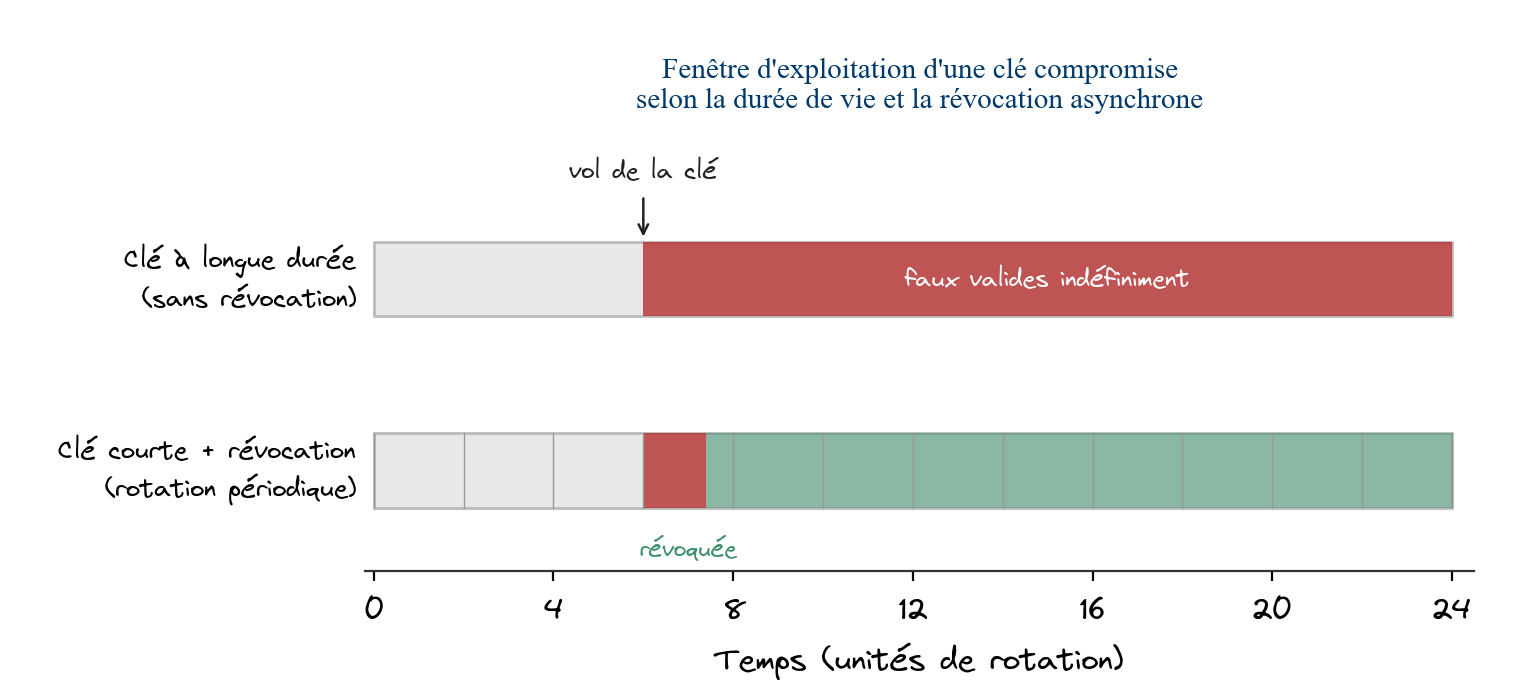
\includegraphics[width=0.80\linewidth]{figures/fig_keywindow.png}
\caption{Fenêtre d'exploitation d'une clé volée. Sans révocation, un vol expose des faux valides indéfiniment~; la rotation courte combinée à la révocation asynchrone borne cette fenêtre à quelques unités de rotation.}
\end{figure}

Le protocole RFC~3161 exige, pour produire un jeton d'horodatage, une interrogation en ligne d'une autorité d'horodatage~: un Bureau de Contrôle Technique sans connectivité sur un chantier isolé ne peut pas l'invoquer au moment même de l'essai. ICES retient donc un \textbf{horodatage en deux paliers}, plutôt que de prétendre à tort qu'un mécanisme intrinsèquement en ligne fonctionne hors-ligne. Le \textbf{palier~1}, disponible partout, signe localement le digest avec l'horloge du dispositif de signature elle-même attestée (section~\ref{sec:profils})~: la date qui en résulte a la force probante de l'horloge matérielle du dispositif, suffisante pour la majorité des usages. Le \textbf{palier~2}, renforcement optionnel, ancre ce même digest auprès d'une autorité d'horodatage RFC~3161 et du journal de transparence dès que le signataire retrouve une connectivité, ce qui donne au sceau une preuve de date indépendante de l'horloge locale. Un sceau de palier~1 reste pleinement valide~; le palier~2 renforce sa force probante sans conditionner son existence, ce qui résout la contradiction entre exigence d'horodatage fort et fonctionnement hors-ligne en la nommant plutôt qu'en la masquant.

\subsection{Le Manifeste de Projet et la chaîne de garde}\label{sec:garde}

Le registre de confiance établit qu'une clé appartient à un professionnel accrédité. Il n'établit pas, à lui seul, que ce professionnel avait le droit d'intervenir sur \emph{ce projet précis, à cette phase précise}. Un bureau d'études et une entreprise de travaux publics détiennent des clés distinctes, enrôlées séparément~; sans mécanisme additionnel, n'importe quel professionnel accrédité pourrait produire un sceau ICES-As-Built valide sur un projet dont il n'a jamais eu la charge, en usurpant la suite d'un APD qui ne lui appartient pas.

ICES ferme cette faille par un \textbf{Manifeste de Projet}, objet cryptographique distinct émis par l'autorité contractante au moment de l'attribution du marché. Ce manifeste lie l'identifiant public du marché aux clés publiques explicitement autorisées pour chaque phase~: la clé du bureau d'études pour l'APD, la clé de l'entreprise adjudicataire pour l'EXE et l'As-Built, la clé du Bureau de Contrôle Technique pour la co-signature de récolement (section~\ref{sec:oracle}). L'étape~6 de la vérification (section~\ref{sec:verif}) contrôle ce manifeste~: un sceau signé par une clé enrôlée mais non autorisée pour ce projet et cette phase est rejeté, quand bien même la signature serait mathématiquement correcte et la clé parfaitement valide dans le registre général. Le schéma complet du Manifeste de Projet est publié en annexe~\ref{sec:spec-schema}.

\subsection{Profils de sécurité des signataires}\label{sec:profils}

La garantie d'attribution ne vaut que ce que vaut la protection de la clé privée du signataire. Un fichier de clé stocké sans chiffrement sur un poste partagé par plusieurs employés d'un bureau d'études annule la garantie d'attribution sans que rien, dans le sceau produit, ne le révèle~: la signature reste mathématiquement valide, mais elle n'identifie plus fiablement une personne. ICES publie, en complément de la spécification, des \textbf{profils de sécurité minimaux recommandés} par catégorie de signataire~: une clé matérielle de type carte à puce ou jeton USB (YubiKey ou équivalent) pour les bureaux d'études et les entreprises, un dispositif de signature renforcé pour les Bureaux de Contrôle Technique compte tenu du poids probant particulier de leur co-signature de récolement (section~\ref{sec:oracle}). Ces profils ne sont pas imposés par la cryptographie elle-même, qui accepte n'importe quelle clé Ed25519 valide~; ils sont une recommandation opérationnelle explicite, dont l'absence de respect reste un risque assumé par le signataire, pas un défaut du protocole.

Cette même section traite la répudiation~: un signataire qui prétend qu'une signature ne provient pas de lui doit pouvoir le démontrer, faute de quoi n'importe quel professionnel pourrait renier après coup un sceau gênant. La combinaison de la fenêtre de rotation courte (section~\ref{sec:cles}), de la révocation d'urgence et de l'obligation de signalement immédiat d'un vol de dispositif limite ce risque~: un signataire qui découvre le vol de son dispositif dispose d'un canal de révocation d'urgence, traité en section~\ref{sec:incident}, qui invalide immédiatement les sceaux futurs sans annuler les sceaux passés antérieurs au vol.

\subsection{Architecture de la clé racine}\label{sec:racine}

\begin{center}
\begin{tikzpicture}[node distance=1.4cm, every node/.style={font=\excalifont\small}]
  \node[draw=rouge, thick, rounded corners, fill=rouge!6, minimum width=4.6cm, minimum height=1.3cm, align=center] (root) {Clé racine (seuil 3 sur 5)\\hors-ligne, air-gap,\\partage de secret Shamir};
  \node[draw=vertAtlas, thick, rounded corners, fill=vertAtlas!8, minimum width=4.6cm, minimum height=1.3cm, align=center, below=of root] (kms) {Clés opérationnelles\\coffre-fort cloud (KMS),\\rotation périodique};
  \draw[-{Latex[length=2.5mm]}, thick] (root) -- node[right, font=\excalifont\footnotesize] {atteste, rarement} (kms);
  \node[right=1.2cm of kms, draw=intrepid, thick, rounded corners, fill=intrepid!8, minimum width=4.2cm, minimum height=1.3cm, align=center] (bundles) {Signent les bundles\\ICES au quotidien};
  \draw[-{Latex[length=2.5mm]}, thick] (kms) -- (bundles);
\end{tikzpicture}
\end{center}

La clé racine ne signe jamais un bundle directement~; elle n'intervient qu'à de rares occasions pour attester ou faire tourner les clés opérationnelles. La cérémonie de clé racine repose sur un \textbf{partage de secret de Shamir}~\cite{shamir1979} à seuil 3 sur 5~: la clé racine n'existe sous forme reconstituée qu'à l'instant de la cérémonie, tenue sur une machine jamais connectée à internet, et sa reconstitution exige la collusion d'au moins trois des cinq porteurs de parts, un seuil délibérément supérieur au risque de collusion à deux qu'un schéma plus simple laisserait ouvert. Chaque cérémonie, rotation ou attestation de clé opérationnelle est documentée dans un procès-verbal signé par les porteurs présents.

Un vol de clé opérationnelle expose une fenêtre bornée et révocable~; un vol de la clé racine exigerait de compromettre trois porteurs de parts indépendants et la logistique d'une cérémonie physique. Un module matériel de sécurité dédié (HSM physique) offrirait une garantie supplémentaire sur la clé racine elle-même~; ce choix est écarté avant la phase de gouvernance élargie, le coût d'acquisition et d'exploitation d'un HSM certifié dépassant ce que justifie le volume actuel de scellements, et la combinaison cérémonie à seuil plus KMS cloud managé couvrant déjà le scénario de menace réaliste à ce stade. La révision de cet arbitrage est prévue au moment où le volume de bundles scellés le justifiera.

\subsection{Réponse à incident et continuité}\label{sec:incident}

Trois scénarios de défaillance sont anticipés plutôt que découverts en situation de crise. \textbf{Compromission d'une clé opérationnelle}~: révocation immédiate publiée au journal de transparence, propagation asynchrone (section~\ref{sec:cles})~; les sceaux signés avant la compromission restent valides par construction, grâce à l'attestation agrafée. \textbf{Compromission de la clé racine}~: seul scénario justifiant une nouvelle cérémonie complète à seuil~; toutes les clés opérationnelles attestées par l'ancienne racine sont révoquées et ré-attestées sous la nouvelle, un événement rare et coûteux par conception, ce qui est la propriété recherchée pour une clé de cette importance. \textbf{Faille découverte dans l'implémentation de référence}~: procédure de divulgation coordonnée, correctif publié avec un délai de préavis avant divulgation publique, et publication d'un correctif de référence dont la conformité aux vecteurs de test (section~\ref{sec:conformite}) est revérifiée avant diffusion. Dans les trois cas, l'intégrité des sceaux déjà émis n'est jamais rétroactivement remise en cause~: seule la capacité à produire de \emph{nouveaux} sceaux avec la clé ou l'implémentation affectée est suspendue.

%% ═════════════════════════════════════════════════════════════
\section{L'oracle physique~: de la donnée saisie à la réalité du chantier}\label{sec:oracle}

\subsection{Ce que la cryptographie ne peut pas garantir}

Le mécanisme des sections 5 et 6 prouve qu'un document n'a pas été modifié depuis sa signature par une clé identifiée. Il ne prouve rien sur l'exactitude du contenu au moment de la signature. Si une entreprise pose une conduite PN10 dans une tranchée et saisit \enquote{PN16} dans le logiciel qui génère le sceau de récolement, le sceau produit est cryptographiquement valide~: la signature est correcte, la clé est enrôlée, le digest correspond au contenu saisi. Un inspecteur qui vérifie ce sceau hors-ligne obtient un résultat positif, alors que la conduite enterrée ne correspond pas au document. C'est une limite structurelle de toute preuve cryptographique appliquée à des faits du monde physique, connue en sécurité de l'information sous le nom de problème de l'oracle~: aucune signature ne peut garantir la véracité d'une donnée qu'elle n'a fait que sceller.

ICES ne prétend pas résoudre ce problème par des mathématiques supplémentaires. Il le traite par deux mécanismes non cryptographiques~: un tiers indépendant dont la signature engage sa propre responsabilité, et l'ancrage de cette signature à des preuves matérielles difficiles à falsifier.

\subsection{Le témoin tiers et les preuves matérielles attestées}

Le sceau de récolement (ICES-As-Built) n'est jamais généré par l'entreprise adjudicataire seule. Il requiert la co-signature du \textbf{Bureau de Contrôle Technique}, tiers indépendant déjà mandaté dans le dispositif d'assurance décennale de la zone CIMA pour prévenir les aléas techniques et produire les rapports périodiques qui conditionnent l'assurabilité de l'ouvrage. Le BCT ne se contente pas d'attester une déclaration~; il signe qu'il a lui-même collecté une preuve numérique déterminée sur le terrain.

Cette distinction est déterminante~: le BCT n'atteste pas \enquote{je certifie que c'est conforme}, une déclaration d'opinion difficile à contester ou à engager juridiquement. Il atteste \enquote{j'ai personnellement collecté cette preuve numérique à cet instant et cet endroit}, une déclaration de fait, vérifiable indépendamment de son jugement professionnel, et qui engage sa propre responsabilité s'il a falsifié la collecte elle-même plutôt que son interprétation. Un BCT sous pression locale devrait alors falsifier une preuve matérielle, pas seulement signer une opinion complaisante~: le coût et le risque pénal de cette falsification sont d'un ordre différent.

Toutes les preuves de terrain n'ont cependant pas la même valeur, et ce document se garderait de tromperie s'il les traitait comme équivalentes. Une photographie géotaguée prise avec un smartphone générique constitue une donnée \textbf{déclarative}~: la métadonnée EXIF qui porte les coordonnées GPS et l'horodatage est écrite par le système d'exploitation du téléphone, modifiable en quelques secondes par une application de simulation de position avant même la prise de vue. Sceller une telle photo avec la même rigueur cryptographique qu'une preuve matérielle ne rend pas la photo plus fiable~: cela scelle parfaitement une donnée qui a pu être falsifiée à la source, un habillage cryptographique qui masquerait la faiblesse plutôt que de la corriger.

\begin{figure}[H]\centering
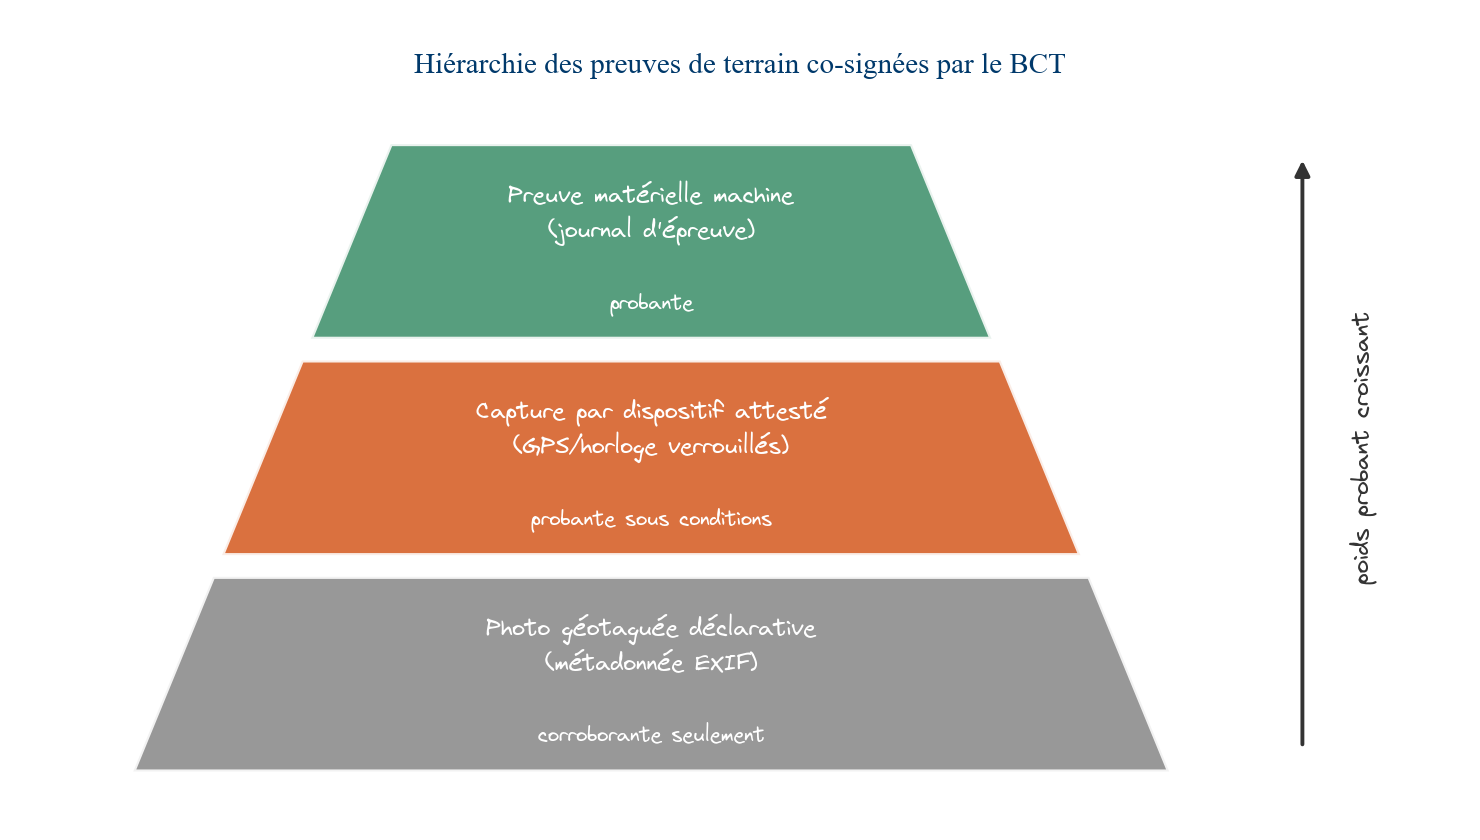
\includegraphics[width=0.72\linewidth]{figures/fig_evidence.png}
\caption{Hiérarchie des preuves de terrain que le BCT peut co-signer. Le poids probant croît avec le niveau d'attestation matérielle, de la simple métadonnée déclarative à la preuve produite par un instrument dont l'horloge et la position échappent au contrôle du signataire.}
\end{figure}

ICES distingue donc trois niveaux de preuve. Une \textbf{photo géotaguée déclarative} reste admissible comme pièce corroborante, jamais comme pièce probante isolée. Une \textbf{capture par dispositif attesté}, application de constat numérique qui verrouille la puce GPS et l'horloge réseau du terminal au moment de la prise de vue et signe la capture elle-même sur le dispositif, sur le modèle des applications de constat d'huissier numérique déjà utilisées dans d'autres contentieux, élève la preuve à un niveau probant sous condition d'utiliser un dispositif certifié. Une \textbf{preuve matérielle produite par un instrument de mesure}, la courbe de montée en pression enregistrée directement par la machine d'épreuve, dont le journal d'enregistrement est intrinsèque à l'appareil et non modifiable par l'opérateur qui le lit, ou le numéro de lot rapproché électroniquement du bordereau de livraison du fournisseur, constitue le niveau le plus probant~: l'instrument, pas l'opérateur, est la source de la donnée. La feuille de route (section~\ref{sec:feuille-de-route}) conditionne la montée en exigence contractuelle de ce niveau de preuve à la disponibilité d'applications de constat certifiées dans la sous-région, une dépendance que ce document nomme plutôt que d'ignorer.

\subsection{De la preuve à la sanction}

Ce mécanisme ne rend pas la collusion impossible. Il la rend plus coûteuse, plus difficile à dissimuler, et il transforme sa découverte en preuve exploitable devant un tribunal ou un assureur, plutôt qu'en simple soupçon, à condition que le niveau de preuve mobilisé corresponde à l'enjeu du contrôle. La section~\ref{sec:juridique} détaille comment cette chaîne de preuve se connecte à la responsabilité décennale et à l'exclusion de garantie pour faute dolosive.

%% ═════════════════════════════════════════════════════════════
\section{Déterminisme et durée de vie du dossier scellé}\label{sec:determinisme}

\subsection{Ce qu'ICES scelle réellement}

Une infrastructure hydraulique a une durée de vie de plusieurs décennies. Si le sceau ne restait valide qu'en supposant qu'un ordinateur de 2066 puisse rejouer un calcul flottant identique bit pour bit à celui de 2026, la garantie serait fragile~: une évolution de compilateur, de système d'exploitation ou d'architecture matérielle peut introduire une divergence sur le dernier bit d'un nombre flottant, ce qui suffit à produire un hash SHA3 totalement différent.

ICES ne repose pas sur cette hypothèse. \textbf{Le sceau porte sur le dossier stocké, pas sur la capacité à recalculer ce dossier.} Vérifier un sceau, tel que décrit en section~\ref{sec:verif}, consiste à contrôler une signature sur un préimage figé, une opération purement combinatoire sur des octets fixes, qui ne relance jamais le solveur hydraulique et n'a donc aucune sensibilité aux flottants. La canonicalisation par troncature de précision (section~\ref{sec:canon}) a déjà éliminé, avant même le premier hachage, les divergences de dernier bit qu'un calcul natif introduirait~: un contentieux en 2066 n'a pas besoin de recalculer un flottant natif identique, il compare une signature à un dossier déjà figé.

\subsection{Reproductibilité, une garantie distincte et bornée}

Un besoin distinct subsiste~: pouvoir rejouer un calcul pour vérifier que le moteur n'a pas menti sur ses propres résultats, au-delà de la simple vérification de signature. Cette reproductibilité est une garantie séparée de l'intégrité du dossier, et ICES la traite comme telle, sans promettre qu'elle tienne indéfiniment.

L'exécution reproductible s'appuie sur une compilation en \textbf{WebAssembly}, dans un environnement \textbf{WASI en profil déterministe strict}~\cite{wasi}, qui neutralise les sources classiques de non-déterminisme d'un exécutable natif~: appels d'horloge système, générateurs d'aléa non graine, ordre d'itération non spécifié sur certaines structures de données. Le toolchain exact (image de compilation, version du moteur) est archivé aux côtés du dossier scellé. Cette reproductibilité est garantie \textbf{au sein d'une version majeure du moteur}, pour la durée où IntrepidCore maintient activement le toolchain archivé correspondant~; elle n'est pas revendiquée comme une propriété éternelle et indépendante de toute maintenance. C'est une différence assumée avec un engagement de bit-exactness inconditionnel sur plusieurs décennies, qui serait techniquement intenable. L'archive elle-même suit une doctrine de préservation numérique standard, migration périodique de format et duplication géographique, distincte de la garantie de validité du sceau, qui ne dépend pas, on l'a vu, de la capacité à recalculer.

\subsection{Agilité cryptographique et menace à long terme}\label{sec:pq}

Une infrastructure scellée aujourd'hui peut rester en service au-delà de 2060. Ed25519 repose sur la difficulté du logarithme discret sur courbe elliptique, un problème qu'un ordinateur quantique suffisamment puissant résoudrait efficacement par l'algorithme de Shor~; SHA3-256 n'est, par comparaison, qu'affaibli par l'algorithme de Grover, sa résistance aux collisions restant de l'ordre de 128 bits, un niveau encore considéré sûr. La menace porte donc spécifiquement sur la \textbf{signature}, pas sur le hachage, et son horizon réaliste, sur la base des estimations publiques de l'informatique quantique~\cite{nistpqc}, se situe au plus tôt dans les années 2035 à 2045~: une fenêtre lointaine, mais pas hors du champ de vie d'une infrastructure hydraulique scellée aujourd'hui.

\begin{figure}[H]\centering
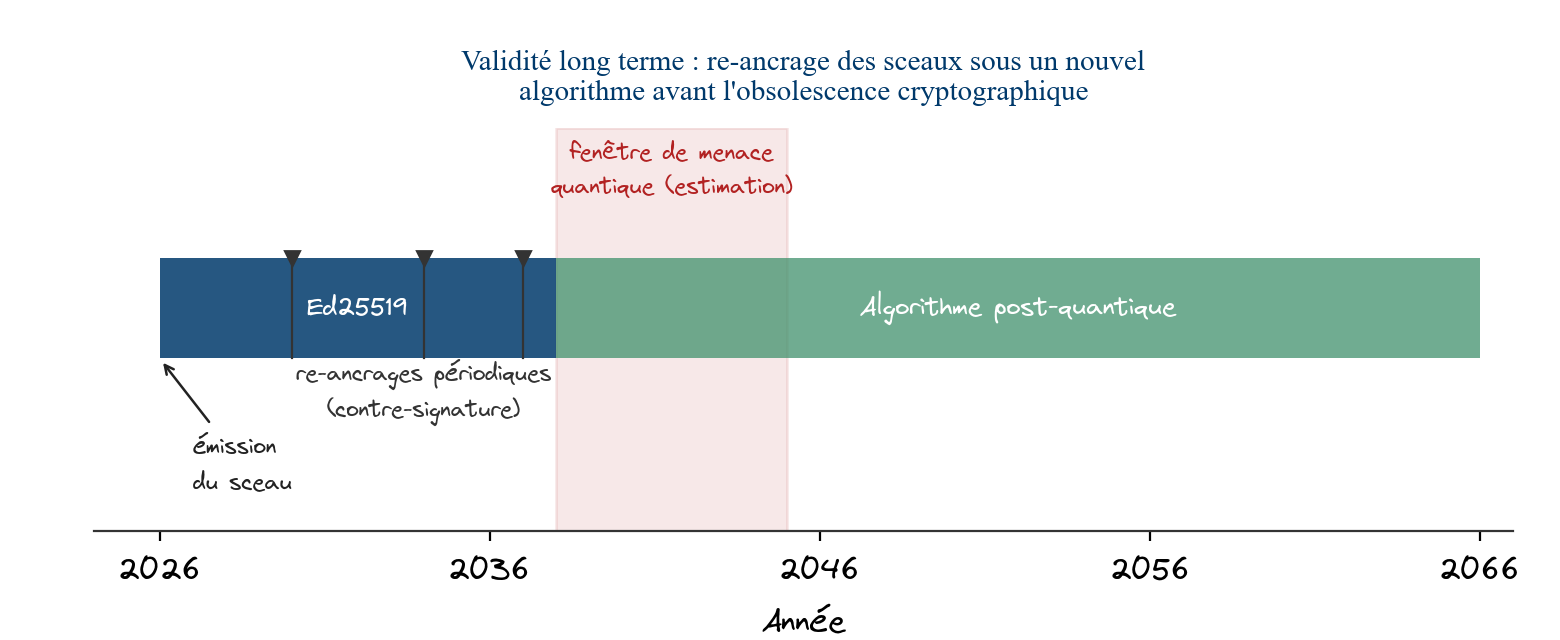
\includegraphics[width=0.86\linewidth]{figures/fig_ltv.png}
\caption{Validité long terme d'un sceau~: le format porte un identifiant d'algorithme (agilité cryptographique) et prévoit des re-ancrages périodiques par contre-signature, plutôt qu'une dépendance permanente à un algorithme unique face à l'obsolescence cryptographique.}
\end{figure}

ICES traite cette menace par deux dispositions, plutôt que par le silence. D'abord, le format du sceau porte un \textbf{identifiant d'algorithme explicite} (agilité cryptographique)~: un nouveau profil s'ajoute au standard sans invalider les sceaux existants, dont le champ d'algorithme reste correctement daté. Ensuite, un mécanisme de \textbf{re-ancrage périodique}, sur le modèle des enregistrements de preuve normalisés (\emph{Evidence Records}, RFC~4998)~\cite{rfc4998}, permet de contre-signer un lot de sceaux existants sous un nouvel algorithme avant que l'ancien ne devienne cassable, prolongeant leur validité sans en altérer le contenu. Une veille sur la standardisation post-quantique du NIST~\cite{nistpqc} est intégrée à la feuille de route (section~\ref{sec:feuille-de-route})~; ce document ne fixe pas d'échéance ferme de migration, faute de visibilité suffisante à ce jour sur le calendrier réel de la menace, mais engage le principe d'agilité qui rend cette migration possible sans réécriture du standard.

\subsection{Synthèse~: ce que la couche technique couvre, et ne couvre pas}

\begin{figure}[H]\centering
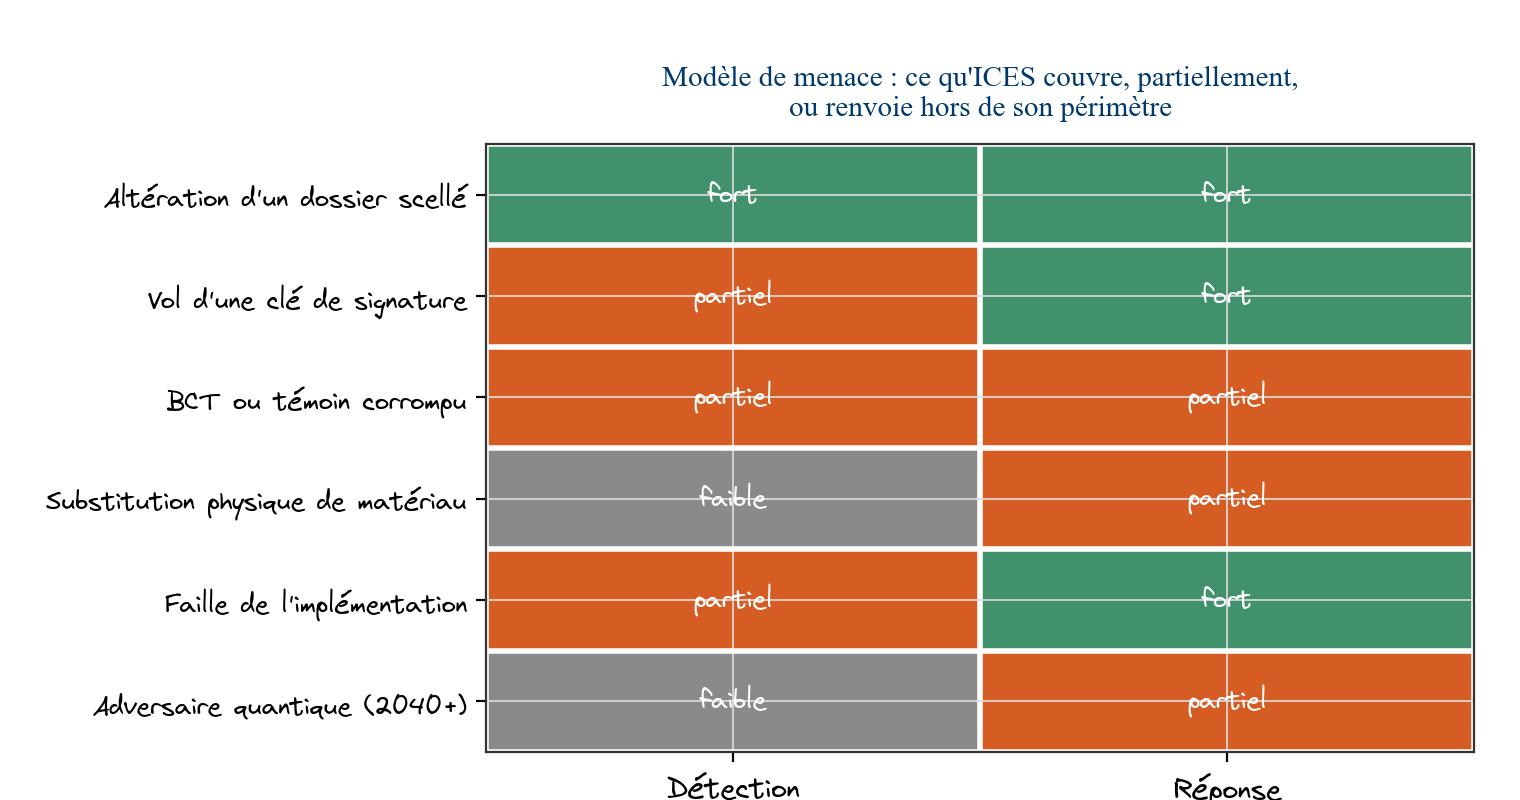
\includegraphics[width=0.86\linewidth]{figures/fig_threat.png}
\caption{Couverture du modèle de menace par les mécanismes décrits aux sections~\ref{sec:anatomie} à~\ref{sec:determinisme}. La détection et la réponse sont fortes pour l'altération numérique et le vol de clé~; elles restent partielles ou faibles pour la substitution physique et la menace quantique, dont le traitement dépend d'acteurs et de délais hors du seul contrôle cryptographique.}
\end{figure}

%% ═════════════════════════════════════════════════════════════
\section{De la preuve à la responsabilité juridique}\label{sec:juridique}

\subsection{Cachet avancé, pas qualifié~: ce que cela change devant un juge}

ICES est aujourd'hui un cachet électronique avancé au sens du droit UEMOA de la dématérialisation~\cite{uemoa2023}, pas un cachet ou une signature qualifiée. Un cachet qualifié bénéficie d'une présomption de fiabilité~: le juge le tient pour vrai par défaut, et c'est à la partie qui le conteste d'apporter la preuve contraire. Un cachet avancé ne bénéficie pas de cette présomption~: en cas de contestation, c'est à la partie qui s'appuie sur le sceau, généralement l'administration, d'établir la fiabilité de la cryptographie sous-jacente, potentiellement au prix d'une bataille d'experts. Cette distinction n'est pas un détail de qualification~: elle détermine qui porte la charge de la preuve devant un tribunal. L'obtention d'une accréditation auprès d'un Prestataire de Services de Confiance Qualifié (PSCQ) est un jalon explicite de la feuille de route (section~\ref{sec:feuille-de-route}), pas un fait acquis à ce jour. L'absence de qualification renforce, par ailleurs, l'intérêt d'un audit cryptographique indépendant de l'implémentation de référence (section~\ref{sec:conformite})~: publié et daté, il constitue l'élément que l'administration produira en première ligne d'une éventuelle bataille d'experts, plutôt que de découvrir cette nécessité au moment du contentieux.

\subsection{Le contrat comme substitut, en attendant la présomption légale}

En l'absence de présomption légale, la force du sceau repose sur le droit du contrat plutôt que sur une qualification cryptographique. Le CCTP fait de la conformité ICES une spécification technique substantielle~; le CCAP conditionne les décomptes de paiement et la réception provisoire à la production d'un sceau ICES-As-Built cohérent avec l'enveloppe ICES-APD, dans une tolérance définie contractuellement~; toute altération avérée du protocole est qualifiée contractuellement de pratique frauduleuse au sens des Directives UEMOA, ouvrant la voie à la résiliation aux torts exclusifs et à la saisie de la caution de bonne exécution.

La robustesse probante du sceau devant un juge est en outre renforcée par le fait que ses primitives cryptographiques sont des standards publics (section~\ref{sec:primitives})~: l'administration n'a pas à faire valoir la fiabilité d'un algorithme propriétaire d'IntrepidCore, elle peut s'appuyer sur des normes internationalement reconnues et déjà éprouvées dans d'innombrables systèmes indépendants.

\subsection{Le bâton~: l'exclusion de garantie pour faute dolosive}

Le Code CIMA, applicable dans l'ensemble de l'espace CIMA, contient une disposition d'ordre public~: l'assureur ne répond pas des pertes provenant d'une faute intentionnelle ou dolosive de l'assuré~\cite{cima2012}. Si le CCAP impose le respect de l'enveloppe ICES-APD et qu'une entreprise falsifie délibérément un matériau ou dissimule cette substitution dans le Dossier de Récolement, la rupture de la chaîne cryptographique constitue une preuve techniquement incontestable de cette dissimulation.

Cette preuve doit toutefois être qualifiée avec précision, sans quoi le raisonnement juridique excède ce que la technique établit. Un sceau rompu, ou l'absence d'un sceau ICES-As-Built cohérent avec l'ICES-APD, prouve une \textbf{altération} du dossier. Il ne prouve pas, à lui seul, une \textbf{intention} de tromper~: la qualification de faute dolosive suppose la démonstration d'une volonté délibérée, que la partie adverse peut contester en invoquant une erreur de manipulation, une défaillance logicielle non fautive, ou une compromission de clé dont le signataire n'est pas responsable. Le sceau ne se substitue donc pas à la démonstration de l'intention~; il en \textbf{facilite radicalement l'établissement}, en écartant d'emblée la défense la plus fréquente en pratique, l'ignorance ou l'absence de preuve de l'altération elle-même, et en déplaçant le débat contentieux du fait matériel, difficile à établir sans le sceau, vers la seule question de l'intention. Une analyse jurisprudentielle approfondie de la qualification de faute dolosive dans l'espace CIMA, avec un cabinet spécialisé, reste un chantier ouvert de la feuille de route (section~\ref{sec:feuille-de-route}), ce document se limitant à l'articulation de principe entre la preuve technique et la qualification juridique.

Une fois l'intention établie par ailleurs, l'assureur décennal peut opposer une exclusion de garantie totale sur le fondement de la faute dolosive~: l'entreprise fautive assume seule la réparation, et la faute dolosive permet de lever le voile social pour exposer le patrimoine personnel des dirigeants.

L'engagement du Bureau de Contrôle Technique dans ce dispositif (section~\ref{sec:oracle}) suppose, en miroir, qu'il puisse assurer ce nouveau rôle de témoin cryptographique au titre de sa responsabilité civile professionnelle. Les polices RC Pro courantes dans la zone CIMA n'ont pas été conçues pour ce rôle spécifique de collecte de preuve numérique attestée, et certaines comportent des clauses limitatives de responsabilité qui pourraient l'exclure. La négociation d'une extension de garantie ou d'un avenant type avec les assureurs professionnels des BCT est une condition pratique de la Phase~3 de la feuille de route (section~\ref{sec:feuille-de-route})~; un BCT dont le risque n'est pas assurable n'a pas d'incitation rationnelle à s'engager, quelle que soit la solidité du mécanisme cryptographique.

\subsection{La carotte~: une prime plutôt qu'une seule punition}

Un mécanisme qui n'agit qu'a posteriori, au moment du sinistre, produit une victoire juridique à coût social élevé~: si l'assureur refuse de payer pour faute dolosive et que l'entreprise fautive fait faillite, le maître d'ouvrage obtient gain de cause en droit sans obtenir le financement de la réparation. ICES doit donc aussi jouer un rôle en amont, au moment de la souscription. Un chantier dont l'intégralité du cycle (APD, EXE, As-Built) est scellée présente, pour l'assureur, un risque d'aléa moral structurellement réduit~: la probabilité qu'un sinistre décennal résulte d'une substitution non détectée diminue mécaniquement. Ce document soutient que les assureurs de la zone CIMA ont un intérêt actuariel direct à proposer des primes réduites ou des franchises préférentielles aux chantiers intégralement certifiés ICES, transformant le sceau en outil de réduction de risque financier reconnu par le marché de l'assurance, et non pas seulement en instrument de sanction après coup.

\subsection{Le financement du sinistre, au-delà de la seule exclusion de garantie}\label{sec:financement}

La question du financement de la réparation quand l'entreprise fautive a disparu ou fait faillite reste ouverte et n'est pas résolue par le sceau lui-même. Les instruments classiques de la commande publique, retenue de garantie renforcée, garantie à première demande, ou fonds de garantie sectoriel abondé par une fraction des primes réduites décrites ci-dessus, restent nécessaires en complément. ICES améliore la détection et la preuve de la faute~; il ne se substitue pas à l'ingénierie financière du risque résiduel.

%% ═════════════════════════════════════════════════════════════
\section{Modèle économique}\label{sec:economie}

\begin{figure}[H]\centering
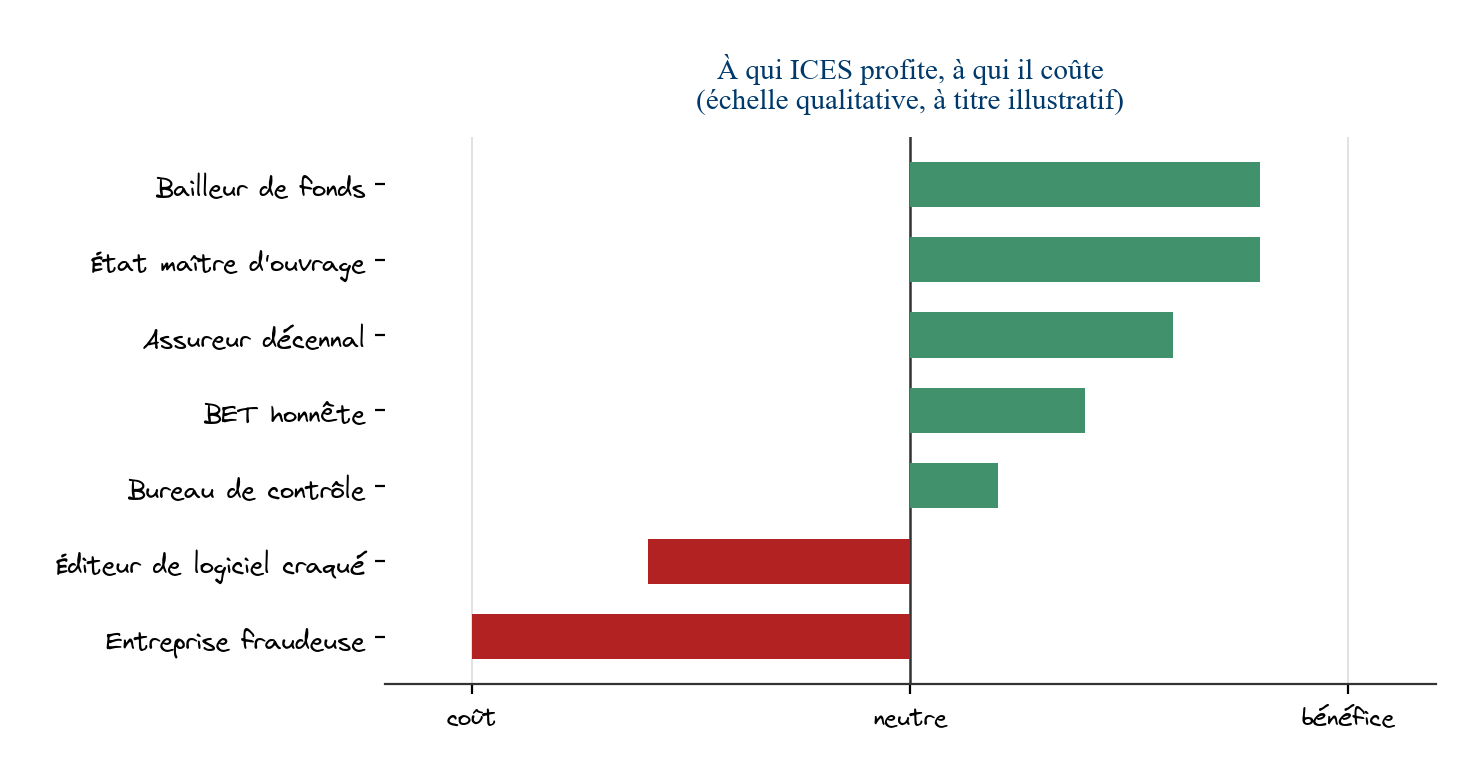
\includegraphics[width=0.80\linewidth]{figures/fig_incentives.png}
\caption{Répartition qualitative des bénéfices et des coûts d'ICES par catégorie d'acteur. Les acteurs dont la valeur repose sur l'opacité ou la fraude en portent le coût~; tous les autres, y compris un éditeur concurrent de bonne foi, y trouvent un bénéfice net.}
\end{figure}

\subsection{Pourquoi le sceau ne peut pas être payant}

Un standard dont la vérification serait payante cesserait d'être un standard de confiance neutre~; il redeviendrait un péage contrôlé par son émetteur, exactement l'objection de monopole traitée en section~\ref{sec:gouvernance}. ICES reste gratuit à produire et à vérifier, y compris avec l'implémentation de référence publiée en Phase~0, qu'un bureau d'études peut utiliser sans acheter aucune licence commerciale. L'entrée dans la conformité ICES est à coût nul.

\subsection{Le passager clandestin, et pourquoi ce document refuse d'y répondre par un verrou}

Un standard réellement ouvert expose IntrepidCore à un risque nommé sans détour~: un éditeur concurrent, y compris l'un des éditeurs dont le logiciel circule aujourd'hui sans licence dans la sous-région (section~\ref{sec:intro}), peut implémenter ICES en quelques semaines et l'adjoindre à son propre outil, sans jamais payer LCPI. La commande publique gagnerait en intégrité~; IntrepidCore ne capterait, dans ce scénario, aucune part de cette victoire.

Une parade technique existe et ce document la rejette explicitement~: filtrer, au niveau du registre de confiance, les sceaux produits par des implémentations dont le \emph{hash de build} ne figure pas sur une liste autorisée. Cette parade est refusée pour trois raisons cumulatives. Premièrement, elle recrée exactement la clause de \enquote{validité de licence du solveur} écartée en section~\ref{sec:gouvernance} comme discriminatoire au sens de l'article 48~: une liste de builds autorisés est une liste de logiciels autorisés, sous un autre nom. Deuxièmement, elle recentralise dans le registre de confiance, conçu comme une couche d'attribution neutre, un pouvoir de police commerciale qui contredit sa raison d'être. Troisièmement, un standard qui se protège de l'implémentation libre par ses concurrents n'est, par définition, pas le standard ouvert que la section~\ref{sec:gouvernance} revendique~: la cohérence doctrinale de ce document interdit d'accepter cette parade au nom d'un intérêt commercial de court terme.

La réponse retenue déplace la question~: si un solveur tiers, gratuit ou piraté, \enquote{suffit} une fois équipé d'un sceau ICES, c'est que LCPI n'apportait pas, sur ce segment, une différenciation suffisante pour justifier son prix, un diagnostic sur LCPI, pas un défaut d'ICES. La valeur commerciale durable d'IntrepidCore ne réside pas dans le contrôle du sceau, cédé par construction, mais dans la qualité du solveur stochastique sur le contexte spécifique que les solveurs déterministes historiques modélisent mal (délestage, intermittence), dans la position de secrétariat technique et d'implémenteur de référence du standard, et dans la couche de services et d'intégration qui l'entoure. Un standard qui profite à un concurrent qui l'adopte de bonne foi est un standard qui a rempli sa mission d'assainissement de la commande publique~; c'est le critère de succès retenu ici, pas un échec à corriger par un verrou.

\subsection{Ce qui est payant~: le solveur, pas le sceau}

La valeur commerciale d'IntrepidCore réside dans le solveur stochastique LCPI, qui optimise le dimensionnement au-delà de ce qu'exige la seule conformité normative, et dont le prix se justifie par l'économie de CAPEX et d'OPEX qu'il produit, jamais par le droit de sceller un calcul.

\begin{figure}[H]\centering
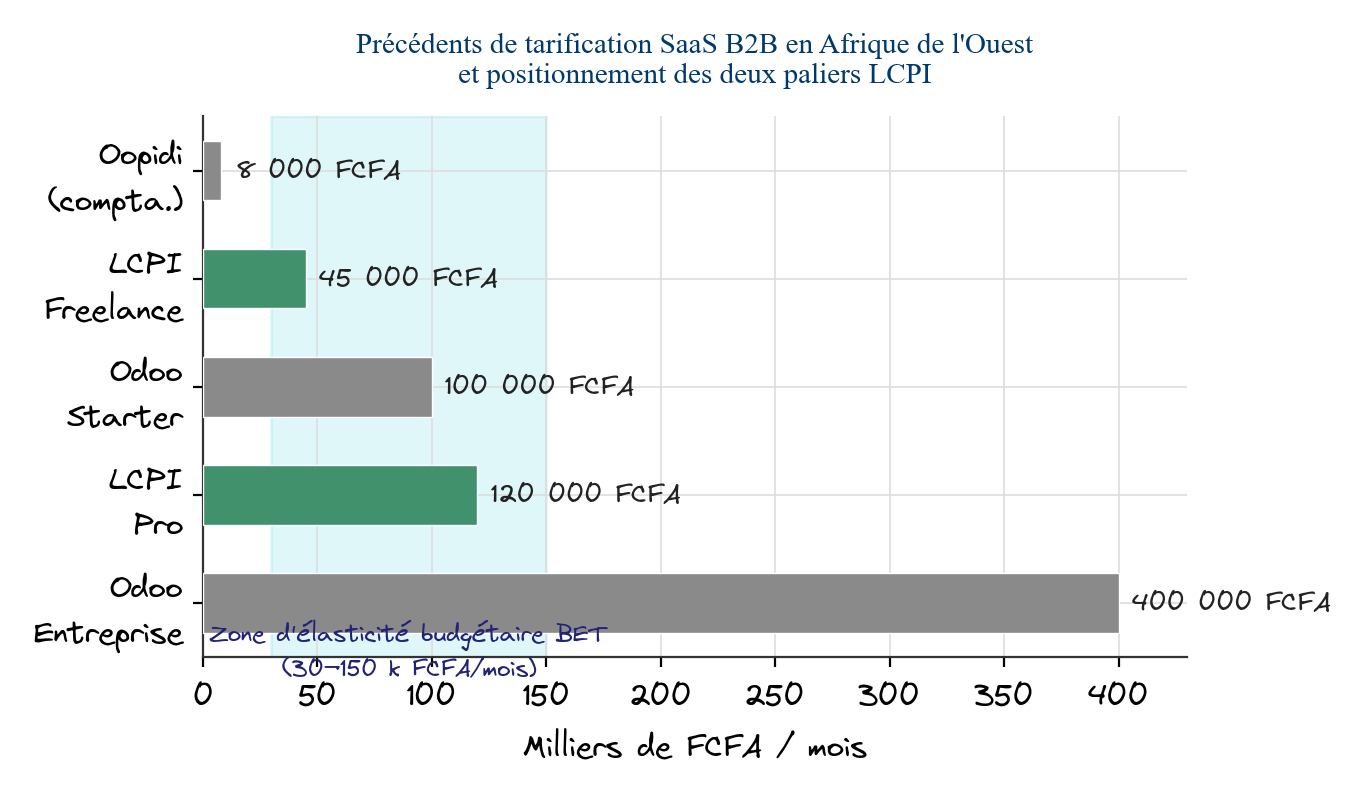
\includegraphics[width=0.78\linewidth]{figures/fig_pricing.png}
\caption{Tarification proposée pour LCPI, comparée à des précédents de SaaS B2B tarifés en FCFA dans la sous-région et à la bande d'élasticité budgétaire mesurée pour un BET.}
\end{figure}

La grille de deux paliers (Freelance, Pro) se situe à l'intérieur de la bande d'élasticité budgétaire mesurée pour un bureau d'études de la sous-région, entre 30\,000 et 150\,000\,FCFA par mois pour un outil métier critique traité comme charge d'exploitation courante. Cette bande, et les deux points de comparaison Oopidi et Odoo, proviennent d'une même enquête de terrain sur la tarification SaaS B2B en zone UEMOA. Aucun de ces montants n'est contractuel~; ils constituent une hypothèse de calibration, à confirmer au moment du premier déploiement réel.

La mission de co-signature du BCT (section~\ref{sec:oracle}) représente un travail et un risque professionnel supplémentaires, sans lesquels le témoin tiers de la chaîne de garde n'a aucune incitation rationnelle à s'engager. Ce document soutient que la \enquote{Mission ICES} doit devenir une ligne budgétaire explicite et rémunérée au bordereau des prix du contrat de contrôle technique, au même titre que les missions normalisées existantes (solidité des ouvrages, sécurité incendie), plutôt qu'une charge implicite ajoutée sans contrepartie à une mission déjà tendue financièrement. Un BCT non rémunéré pour cet acte spécifique de notarisation numérique le traitera, en pratique, avec la même complaisance que les contrôles déjà défaillants que ce document entend corriger.

\subsection{Les Marchés Globaux de Performance~: une destination, pas un point d'entrée}

Le partage de gains issu de l'optimisation stochastique constitue une source de revenu additionnelle envisageable, structurée en Contrat Basé sur la Performance sous le régime des Marchés Globaux de Performance, jamais comme une facture directe d'IntrepidCore indexée sur une économie estimée, ce que le principe de non-contraction budgétaire interdit. Ce mécanisme suppose une capacité contractuelle et d'audit que l'administration locale ne possède pas toujours~: le même document qui décrit, en section~\ref{sec:intro}, une administration incapable de vérifier systématiquement une classe de tuyau ne peut pas raisonnablement présupposer qu'elle pilotera, dès le premier déploiement, un contrat de performance sophistiqué avec intéressement financier.

Ce mécanisme est donc positionné comme une \textbf{destination}, atteignable une fois la maturité contractuelle établie, généralement par l'intermédiaire d'un bailleur de fonds international qui possède déjà une pratique du décaissement basé sur les résultats et peut porter la complexité contractuelle que l'administration locale ne porte pas seule. Le revenu de premier ordre, celui qui ne suppose aucune maturité institutionnelle particulière et qui ne dépend de la matérialisation d'aucun appui bailleur, reste l'abonnement SaaS à tarif fixe décrit ci-dessus~: si l'appui bailleur nécessaire au MGP ne se matérialise jamais sur un marché donné, le modèle économique reste viable sur cette seule base.

\begin{figure}[H]\centering
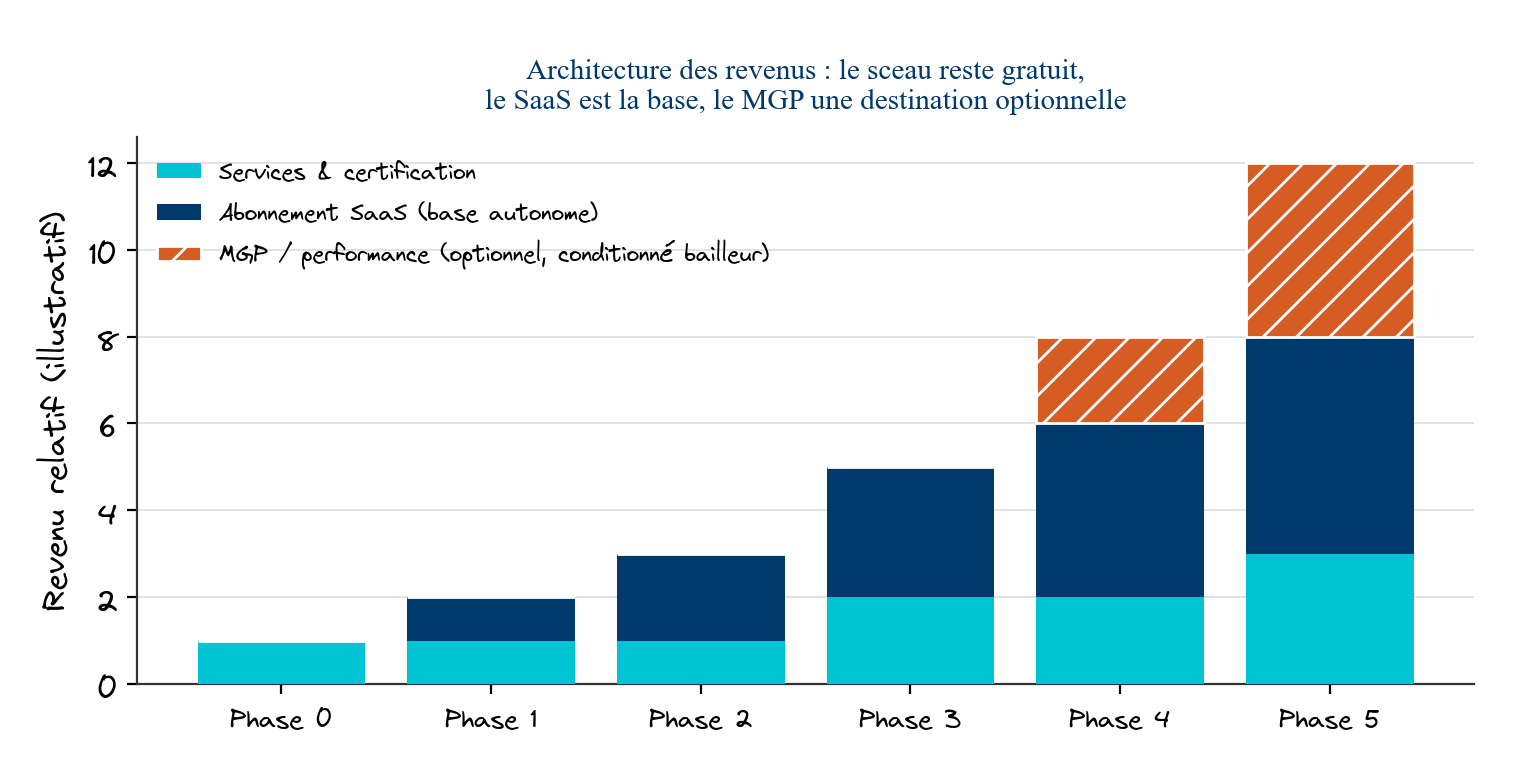
\includegraphics[width=0.84\linewidth]{figures/fig_revenue.png}
\caption{Architecture des revenus par phase de la feuille de route. Le sceau reste gratuit à chaque phase~; l'abonnement SaaS constitue la base autonome de revenu dès la Phase~1~; le Marché Global de Performance n'intervient qu'à partir de la Phase~4, conditionné à la maturité contractuelle d'un bailleur.}
\end{figure}

%% ═════════════════════════════════════════════════════════════
\section{Feuille de route et gouvernance}\label{sec:feuille-de-route}

\begin{figure}[H]\centering
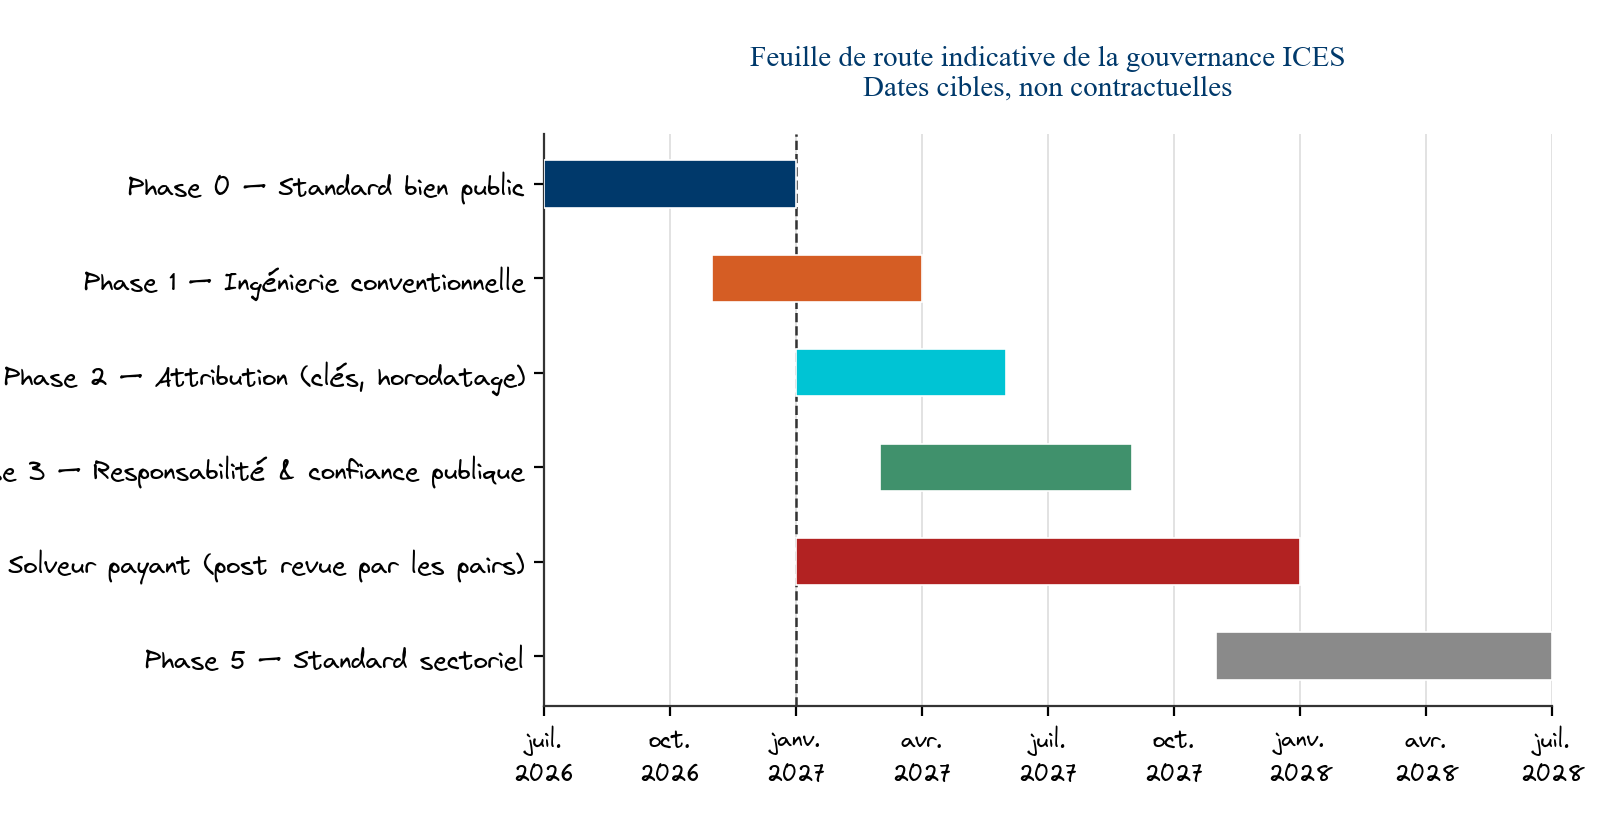
\includegraphics[width=0.92\linewidth]{figures/fig_roadmap.png}
\caption{Feuille de route indicative des six phases de gouvernance décrites ci-dessous. Les dates sont des cibles de planification, non des engagements contractuels.}
\end{figure}

\textbf{Phase~0 — Standard bien public.} Spécification (annexe~\ref{sec:annexe}), vecteurs de test et implémentation de référence sous licence Apache-2.0 publiés, hébergement neutre miroité. Fondation de l'organe de gouvernance, IntrepidCore fondateur et secrétariat technique, marque de conformité et suite de tests maintenues séparément (section~\ref{sec:conformite}).

\textbf{Phase~1 — Ingénierie conventionnelle.} ICES scelle des calculs déterministes normatifs (Fascicule 71, Hardy-Cross), indépendamment de toute validation du moteur stochastique de LCPI. Cette phase découple délibérément l'adoption d'ICES de la maturité scientifique de LCPI, traitée séparément ci-dessous. Le format du sceau porte, dès cette phase, un numéro de version~: un sceau de Phase~1 reste vérifiable indéfiniment, les phases suivantes ajoutant des champs sans jamais invalider un format antérieur.

\textbf{Phase~2 — Attribution.} Déploiement des clés opérationnelles à durée de vie courte, de l'horodatage en deux paliers et du journal de révocation asynchrone (section~\ref{sec:cles}), des profils de sécurité des signataires (section~\ref{sec:profils}), et de la cérémonie de clé racine à seuil (section~\ref{sec:racine}).

\textbf{Phase~3 — Responsabilité et confiance publique.} Déploiement du Manifeste de Projet et de la chaîne de garde (section~\ref{sec:garde}), intégration de la co-signature du Bureau de Contrôle Technique (section~\ref{sec:oracle}) dans le flux de récolement une fois la question de son assurabilité résolue (section~\ref{sec:juridique}), et transfert progressif du registre de confiance vers une autorité publique ou professionnelle, avec le consortium de gouvernance comme détenteur de repli (section~\ref{sec:confiance}).

\textbf{Phase~4 — Solveur payant.} Le moteur stochastique de LCPI devient le produit commercial superposé au sceau gratuit, conditionné par l'achèvement de la revue par les pairs décrite ci-dessous.

\textbf{Phase~5 — Standard sectoriel.} Gouvernance élargie, registre public, audit cryptographique indépendant de l'implémentation de référence réalisé et publié~: ICES entre dans les modèles de dossiers d'appel d'offres via la clause \enquote{ou équivalent} de l'article 48, sur un fondement juridique consolidé.

\subsection{L'état de validation scientifique du moteur stochastique, sans ambiguïté}

Le moteur stochastique de LCPI, distinct du mécanisme de scellement ICES lui-même, est aujourd'hui calibré sur un périmètre géographique restreint et n'a pas encore été soumis à revue par les pairs. La soumission d'un article et la publication d'un préprint sont prévues pour la fin de l'année 2026 et le début de l'année 2027, avant toute exploitation commerciale à grande échelle du volet stochastique. Au moment de la publication de ce document, cette validation par la communauté scientifique n'est pas acquise~: c'est un jalon à venir, pas un fait établi. Cette incertitude ne porte pas sur le mécanisme de scellement ICES lui-même, dont les primitives cryptographiques sont des standards publics indépendants de LCPI et déjà éprouvés, ce qui justifie le séquençage de la Phase~1~: ICES peut s'adopter avant que le solveur stochastique ait fait ses preuves, parce que les deux ne partagent pas la même base de crédibilité.

Toute affirmation de robustesse du mécanisme cryptographique repose, dans ce document, sur des sources externes vérifiables par un tiers, spécifications IETF et NIST, articles de cryptographie publiés, plutôt que sur une auto-évaluation interne à IntrepidCore. C'est la revendication que ce document retient~: vérifiable par des tiers, pas affirmée par son auteur.

%% ═════════════════════════════════════════════════════════════
\section{Limites et non-objectifs explicites}\label{sec:limites}

Cette section énonce, sans les minimiser, ce qu'ICES ne fait pas.

\textbf{ICES ne détecte pas une substitution physique au moment où elle survient.} Il rend cette substitution attribuable et coûteuse à dissimuler durablement (section~\ref{sec:oracle}), il ne l'empêche pas mécaniquement.

\textbf{ICES ne remplace pas le contrôle technique réglementaire.} Le Bureau de Contrôle Technique reste l'acteur de terrain~; ICES rend sa mission plus difficile à contourner, il n'en dispense pas, et sa capacité à assumer ce rôle dépend de conditions économiques et assurantielles qui ne relèvent pas d'ICES (section~\ref{sec:juridique}).

\textbf{ICES ne constitue pas, à ce jour, une signature électronique qualifiée.} La présomption légale de fiabilité qui accompagne une telle qualification n'existe pas encore pour ICES (section~\ref{sec:juridique}).

\textbf{ICES n'est pas une garantie de qualité d'ingénierie.} Un calcul rigoureusement scellé peut reposer sur des hypothèses hydrauliques erronées ou sous-dimensionnées~; le sceau atteste l'intégrité et l'attribution d'un résultat, jamais sa justesse technique.

\textbf{ICES ne résout pas le financement d'un sinistre lorsque l'entreprise responsable a disparu.} Cette limite est traitée par les instruments d'assurance et de garantie décrits en section~\ref{sec:financement}, pas par le sceau lui-même.

\textbf{ICES ne dispense pas d'une gouvernance de clé rigoureuse.} La sécurité du dispositif dépend entièrement de la qualité d'exécution du registre de confiance, du Manifeste de Projet et de la cérémonie de clé racine décrits en section~\ref{sec:confiance}~; un registre mal opéré ou un dispositif de signature mal protégé (section~\ref{sec:profils}) annule la garantie d'attribution, quelle que soit la solidité des primitives cryptographiques sous-jacentes.

\textbf{ICES n'établit pas, à lui seul, l'authenticité d'une preuve de terrain.} La hiérarchie des preuves décrite en section~\ref{sec:oracle} distingue ce qui est probant de ce qui n'est que corroborant~; sceller une donnée falsifiée à la source ne la rend pas plus vraie.

Un lecteur qui cherche une solution technique unique éliminant la fraude d'ingénierie ne la trouvera pas dans ce document, parce qu'une telle solution n'existe pas. Ce que ce document propose est un mécanisme qui déplace le coût de la fraude, de la dissimulation facile vers l'attribution personnelle et opposable, et qui s'appuie, pour le reste, sur les institutions existantes de contrôle et de responsabilité plutôt que sur des mathématiques.

%% ═════════════════════════════════════════════════════════════
\section{Annexe technique}\label{sec:annexe}

Cette annexe rassemble la spécification de mise en œuvre~: tant qu'un dépôt de spécification dédié n'a pas été constitué (Phase~0, section~\ref{sec:feuille-de-route}), elle en constitue la source de vérité unique. Le contenu ci-dessous est normatif~; une implémentation qui s'en écarte n'est pas conforme, indépendamment de ce qu'elle revendique.

\subsection{Schéma du MissionBundle}\label{sec:spec-schema}

\begin{table}[H]\centering\small
\caption{Champs principaux d'un bundle ICES}
\begin{tabularx}{\linewidth}{@{}p{2.5cm}p{3.2cm}X@{}}
\toprule
\textbf{Bloc} & \textbf{Champs} & \textbf{Contenu} \\
\midrule
\texttt{inputs} & \texttt{topology}, \texttt{materials}, \texttt{diameters\_mm} & Topologie du réseau, matériaux déclarés, diamètres nominaux retenus à l'étude \\
\texttt{scenario} & \texttt{power\_outage}, \texttt{demand\_profile} & Hypothèses utilisées pour le calcul (délestage, demande) \\
\texttt{engine\_version} & \texttt{version}, \texttt{build\_hash} & Identifiant exact de la version du moteur ayant produit le résultat \\
\texttt{outputs} & \texttt{pressures}, \texttt{flows}, \texttt{resilience\_indices} & Pressions et débits calculés, indicateurs retenus \\
\texttt{gates} & \texttt{thresholds}, \texttt{compliance} & Seuils normatifs appliqués et statut de conformité de chaque contrainte \\
\texttt{attestation} & \texttt{signer\_did}, \texttt{timestamp}, \texttt{tier}, \texttt{signature} & Identité du signataire (\texttt{did:key}), horodatage palier 1 ou 2 (section~\ref{sec:cles}), signature Ed25519 \\
\texttt{project\_ref} & \texttt{manifest\_id}, \texttt{phase} & Référence au Manifeste de Projet et phase déclarée (APD, EXE, As-Built) \\
\bottomrule
\end{tabularx}
\end{table}

Extrait normatif du schéma JSON (JSON Schema, Draft 2020-12) du bloc \texttt{attestation}, à titre d'illustration du niveau de précision attendu pour l'ensemble du document~:

\begin{lstlisting}[style=icesjson]
{
  "$id": "https://spec.ices.example/attestation.schema.json",
  "type": "object",
  "required": ["signer_did", "timestamp", "tier", "signature"],
  "properties": {
    "signer_did":  { "type": "string", "pattern": "^did:key:z[1-9A-HJ-NP-Za-km-z]+$" },
    "timestamp":   { "type": "string", "format": "date-time" },
    "tier":        { "type": "integer", "enum": [1, 2] },
    "tsa_token":   { "type": "string", "contentEncoding": "base64",
                     "description": "Jeton RFC 3161, requis si tier = 2" },
    "signature":   { "type": "string", "contentEncoding": "base64" },
    "algorithm":   { "type": "string", "enum": ["ed25519-sha3-256-v1"],
                     "description": "Identifiant d'algorithme, agilite cryptographique (sec. 8.2)" }
  }
}
\end{lstlisting}

\begin{table}[H]\centering\small
\caption{Champs principaux du Manifeste de Projet (section~\ref{sec:garde})}
\begin{tabularx}{\linewidth}{@{}p{2.8cm}X@{}}
\toprule
\textbf{Champ} & \textbf{Contenu} \\
\midrule
\texttt{manifest\_id} & Identifiant public unique du marché, attribué par l'autorité contractante \\
\texttt{issuer\_did} & \texttt{did:key} de l'autorité contractante émettrice du manifeste \\
\texttt{authorized\_keys} & Liste \texttt{\{did, phase\}}~: une entrée par clé autorisée et la phase (APD / EXE / As-Built) pour laquelle elle l'est \\
\texttt{tolerance} & Écart maximal toléré entre sceaux successifs (section~\ref{sec:juridique}), par grandeur \\
\texttt{issued\_at} & Date d'émission, phase d'attribution du marché \\
\bottomrule
\end{tabularx}
\end{table}

\subsection{Table de troncature de précision}\label{sec:spec-precision}

Cette table fixe, de façon exhaustive et non ambiguë, le nombre de décimales retenu par grandeur avant canonicalisation JCS (section~\ref{sec:canon}). Deux implémentations conformes appliquent strictement cette table~; en diverger produit un digest différent pour un même calcul physique.

\begin{table}[H]\centering\small
\caption{Précision fixée par grandeur physique}
\begin{tabularx}{\linewidth}{@{}Xrl@{}}
\toprule
\textbf{Grandeur} & \textbf{Décimales} & \textbf{Unité} \\
\midrule
Diamètre nominal & 0 & mm \\
Pression de service & 3 & bar \\
Débit & 4 & m³/h \\
Cote altimétrique & 3 & m \\
Coefficient de rugosité (Hazen-Williams) & 2 & sans dimension \\
Indice de résilience (COT, EENS, LOWLP) & 6 & sans dimension \\
Coordonnée géographique (latitude/longitude) & 7 & degrés décimaux \\
\bottomrule
\end{tabularx}
\end{table}

\subsection{Format de l'état de révocation}\label{sec:spec-revocation}

L'état de révocation synchronisé par le vérificateur (section~\ref{sec:cles}) est une liste plate, conçue pour tenir sur un support de transport minimal~:

\begin{lstlisting}[style=icesjson]
{
  "issued_at": "2026-07-12T00:00:00Z",
  "valid_until": "2026-07-19T00:00:00Z",
  "merkle_root": "3f9a8c...e21b",
  "revoked": [
    { "did": "did:key:z6Mk...9Qh", "revoked_at": "2026-07-10T14:32:00Z", "reason": "key_theft" }
  ]
}
\end{lstlisting}

Le champ \texttt{valid\_until} fixe le seuil de fraîcheur maximal~: un vérificateur dont la dernière synchronisation est postérieure à cette date refuse tout sceau par défaut (\emph{fail-closed}, section~\ref{sec:cles}), plutôt que d'accepter sur la base d'un état potentiellement obsolète. La fenêtre recommandée en Phase~2 est de sept jours~; elle peut être resserrée par une autorité contractante pour des ouvrages à enjeu élevé.

\subsection{Vecteur de test illustratif}

\begin{center}
\begin{termbox}[Exemple illustratif de sortie de l'outil de vérification (format cible)]
\$ ices-verify bundle\_reseau\_zone3.json\\
\ \\
Sceau ICES .......................... CONFORME\\
Digest SHA3-256 .......... 3f9a8c...e21b (32 octets)\\
Signataire .... did:key:z6Mkf5...9Qh (registre : enrôlé)\\
Signature Ed25519 ......................... VALIDE\\
Horodatage RFC 3161 ................. NON CONTESTÉ\\
État de révocation (dernière synchro.) .... À JOUR
\end{termbox}
\end{center}

\subsection{Glossaire}

\begin{table}[H]\centering\small
\begin{tabularx}{\linewidth}{@{}p{3cm}X@{}}
\toprule
\textbf{Terme} & \textbf{Définition} \\
\midrule
APD & Avant-Projet Détaillé, phase d'étude qui fixe le dimensionnement contractuel de l'ouvrage \\
EXE & Études d'Exécution, reprise du dimensionnement par l'entreprise adjudicataire avant travaux \\
BCT & Bureau de Contrôle Technique, tiers indépendant chargé de prévenir les aléas techniques \\
JCS & JSON Canonicalization Scheme, RFC~8785, forme canonique unique d'un document JSON \\
\texttt{did:key} & Identifiant de clé publique auto-descriptif, sans autorité de certification centrale \\
WASI déterministe & Profil d'exécution WebAssembly qui neutralise les sources classiques de non-déterminisme \\
Attestation agrafée & Preuve de validité d'une clé embarquée dans le sceau au moment de la signature \\
Manifeste de Projet & Objet cryptographique liant un marché public aux clés autorisées par phase (section~\ref{sec:garde}) \\
Palier d'horodatage & Niveau de preuve temporelle~: palier~1 (horloge locale attestée, hors-ligne) ou palier~2 (RFC~3161, ancrage réseau) \\
Moniteur tiers & Organisation indépendante qui synchronise et audite publiquement le journal de transparence \\
Partage de Shamir & Schéma cryptographique qui répartit un secret entre plusieurs porteurs, reconstituable à partir d'un seuil~\cite{shamir1979} \\
Agilité cryptographique & Capacité d'un format à identifier son algorithme et à en changer sans invalider les données existantes \\
MGP/PBC & Marché Global de Performance / \emph{Performance-Based Contract}, cadre contractuel autorisant l'intéressement aux économies réalisées \\
PSCQ & Prestataire de Services de Confiance Qualifié, accréditation conférant la présomption légale de fiabilité \\
\bottomrule
\end{tabularx}
\end{table}

\printbibliography

\vspace{0.3cm}\rule{\linewidth}{0.4pt}
\vspace{0.2cm}
\begin{center}\footnotesize\color{gray}
IntrepidCore \textperiodcentered\ Lomé \textperiodcentered\ Livre blanc ICES v3.0
\end{center}
\end{document}
